\chapter{Requirements, Constraints and Design}

In this chapter we will talk about the design of the bootware component and the requirements and constraints that shape it.
We begin with the requirements, which were explicitly given at the beginning of this thesis.
Next, we describe additional constraints which we added to limit the scope of the work.
Then, we explain the design that formed as a result of the limitations that we had.

\section{Requirements}

The main goal of this diploma thesis is to lay a foundation by creating the core design of the bootware.
It was clear from the beginning that, because of the limited time available, not every feature that might be necessary for the full operation can be fully implemented.
Instead, the foundation we develop here should keep future needs in mind and make it simple to extend the bootware when needed.
It is therefore a core requirement to keep the bootware relatively generic and make it extensible where necessary.

It should be extensible in two key areas, namely the support for different cloud providers and for different provisioning engines.
For this diploma thesis, Amazon is the only cloud provider that has to be supported, but it has to be possible to add others in the future.
Concerning provisioning engines, only OpenTOSCA has to be supported for now, but again with the possibility to add more in the future.

It is also important that the bootware is easy to use.
In fact, it should be practically invisible whenever possible.
It should hook into the already existing process of executing a workflow without adding unnecessary interaction steps when possible.
However, It cannot be hidden completely, because the user has to specify a cloud provider and the corresponding log-in credentials somewhere.
The user should also get some feedback about the progress of the deployment because this process might take some time and might seem unresponsive without frequent status updates.

A further requirement is that the bootware should be relatively lightweight and open standards should be used where possible.
In this case, lightweight means that the bootware should be small, independent program that does not require a huge supporting infrastructure to be executed.
It should also be easy to distribute and setup and it has to be able to run on an average personal computer.

\section{Constraints}

The bootware could theoretically be written in any major programming language but we limit our selves to Java.
The reason for this is that all the other SimTech components are written in Java, so by also using Java we fit nicely into this already existing ecosystem.
Additionally, for things like Eclipse integration we would have to use Java anyway.
We also have to keep in mind that the bootware will not be finished with this thesis.
Other people will have to extend it in the future and since Java is common in general, as well as in the SimTech project, it makes sense to use it instead of another programming language.
We can further narrow our use of Java by limiting us to Java 1.6.
This also has to do with the already existing parts of the SimTech project, that are geared towards this version as well.
Using another version of Java could lead to unforeseen incompatibilities.
We also constrain the bootware usage to one bootware per user.
We don't plan for multi-tenancy, i.e. multiple users using the same bootware.
In the next chapter we will also introduce additional constraints that became necessary during the design process and will therefore be explained at the appropriate times.


\section{Design}
\label{design}

In this section we will develop the design of the bootware.
This design is held intentionally abstract.
Specific implementation details will be selected and described in \autoref{selecting}.

\subsection{Component Division}

The first question that has to be answered is whether or not it makes sense to divide the bootware component into two or more cooperating components, i.e. a server client division or a similar structure.
\textcolor{red}{As described in \autoref{related:ondemand} on page \pageref{related:ondemand}, the proposed architecture initially only envisioned one bootware component.
This architecture was expanded with the introduction of the provisioning manager, as described in \autoref{related:dynamic} on page \pageref{related:dynamic}.}
We will now discuss the viability of these architectures.

\subsubsection{Single Local Component}

\begin{figure}[!htbp]
	\centering
	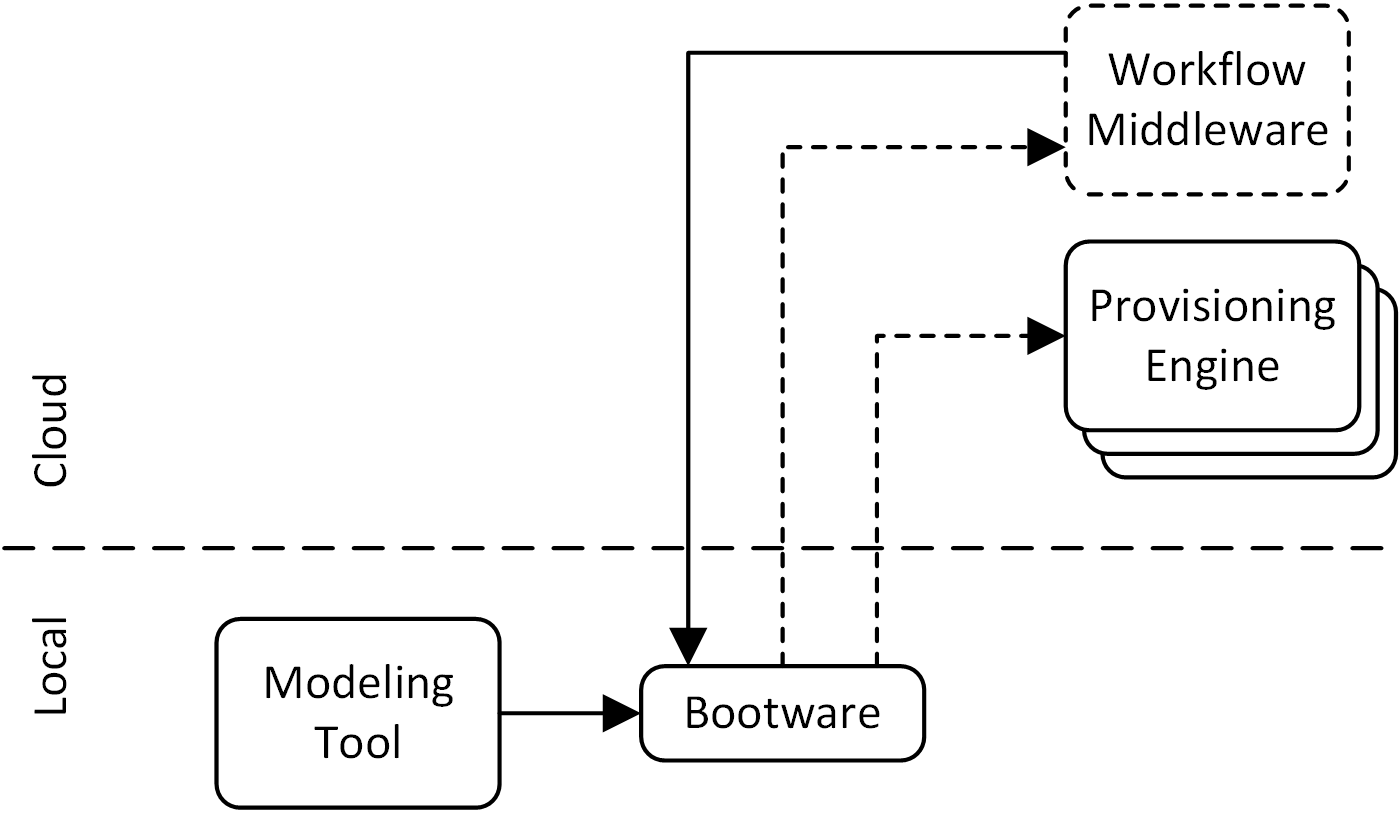
\includegraphics[resolution=600]{design/assets/simple_local}
	\caption{Simplified overview of the single local component architecture}
	\label{image:single_local}
\end{figure}

First we consider the simplest case: A single local component.
In this scenario, all provisioning processes are initiated from a component installed locally on the users machine, alongside or as part of the workflow modeler.

The advantages of this architecture lie in its simplicity.
Only one component has to be created and managed.
We wouldn't have to deal with any cloud environments and each user would have his own personal instance, so multi-tenancy wouldn't be an issue.
There is no possible overlap in functionality, as in a 2-tier architecture (see \autoref{design:division:2tier}) and communication between multiple bootware components doesn't have to be considered.

The disadvantages are caused by the component being local.
Since all the functionality is concentrated in one component, it can become quite large and complicated, which is one thing that should be avoided according to the requirements.
A much bigger problem however is the remote communication happening in this scenario.
All calls to the bootware component from the ESB of the workflow middleware would leave the remote environment.
Also, all calls from the bootware component to the provisioning engines would enter the remote environment.
This type of split communication can be costly and slow, as shown by Li et al.
They compared public cloud providers and measured that intra-datacenter communication can be two to three times faster and also cheaper (often free) compared to inter-datacenter communication~\autocite{cloudcmp}.

\subsubsection{Single Remote Component}

\begin{figure}[!htbp]
	\centering
	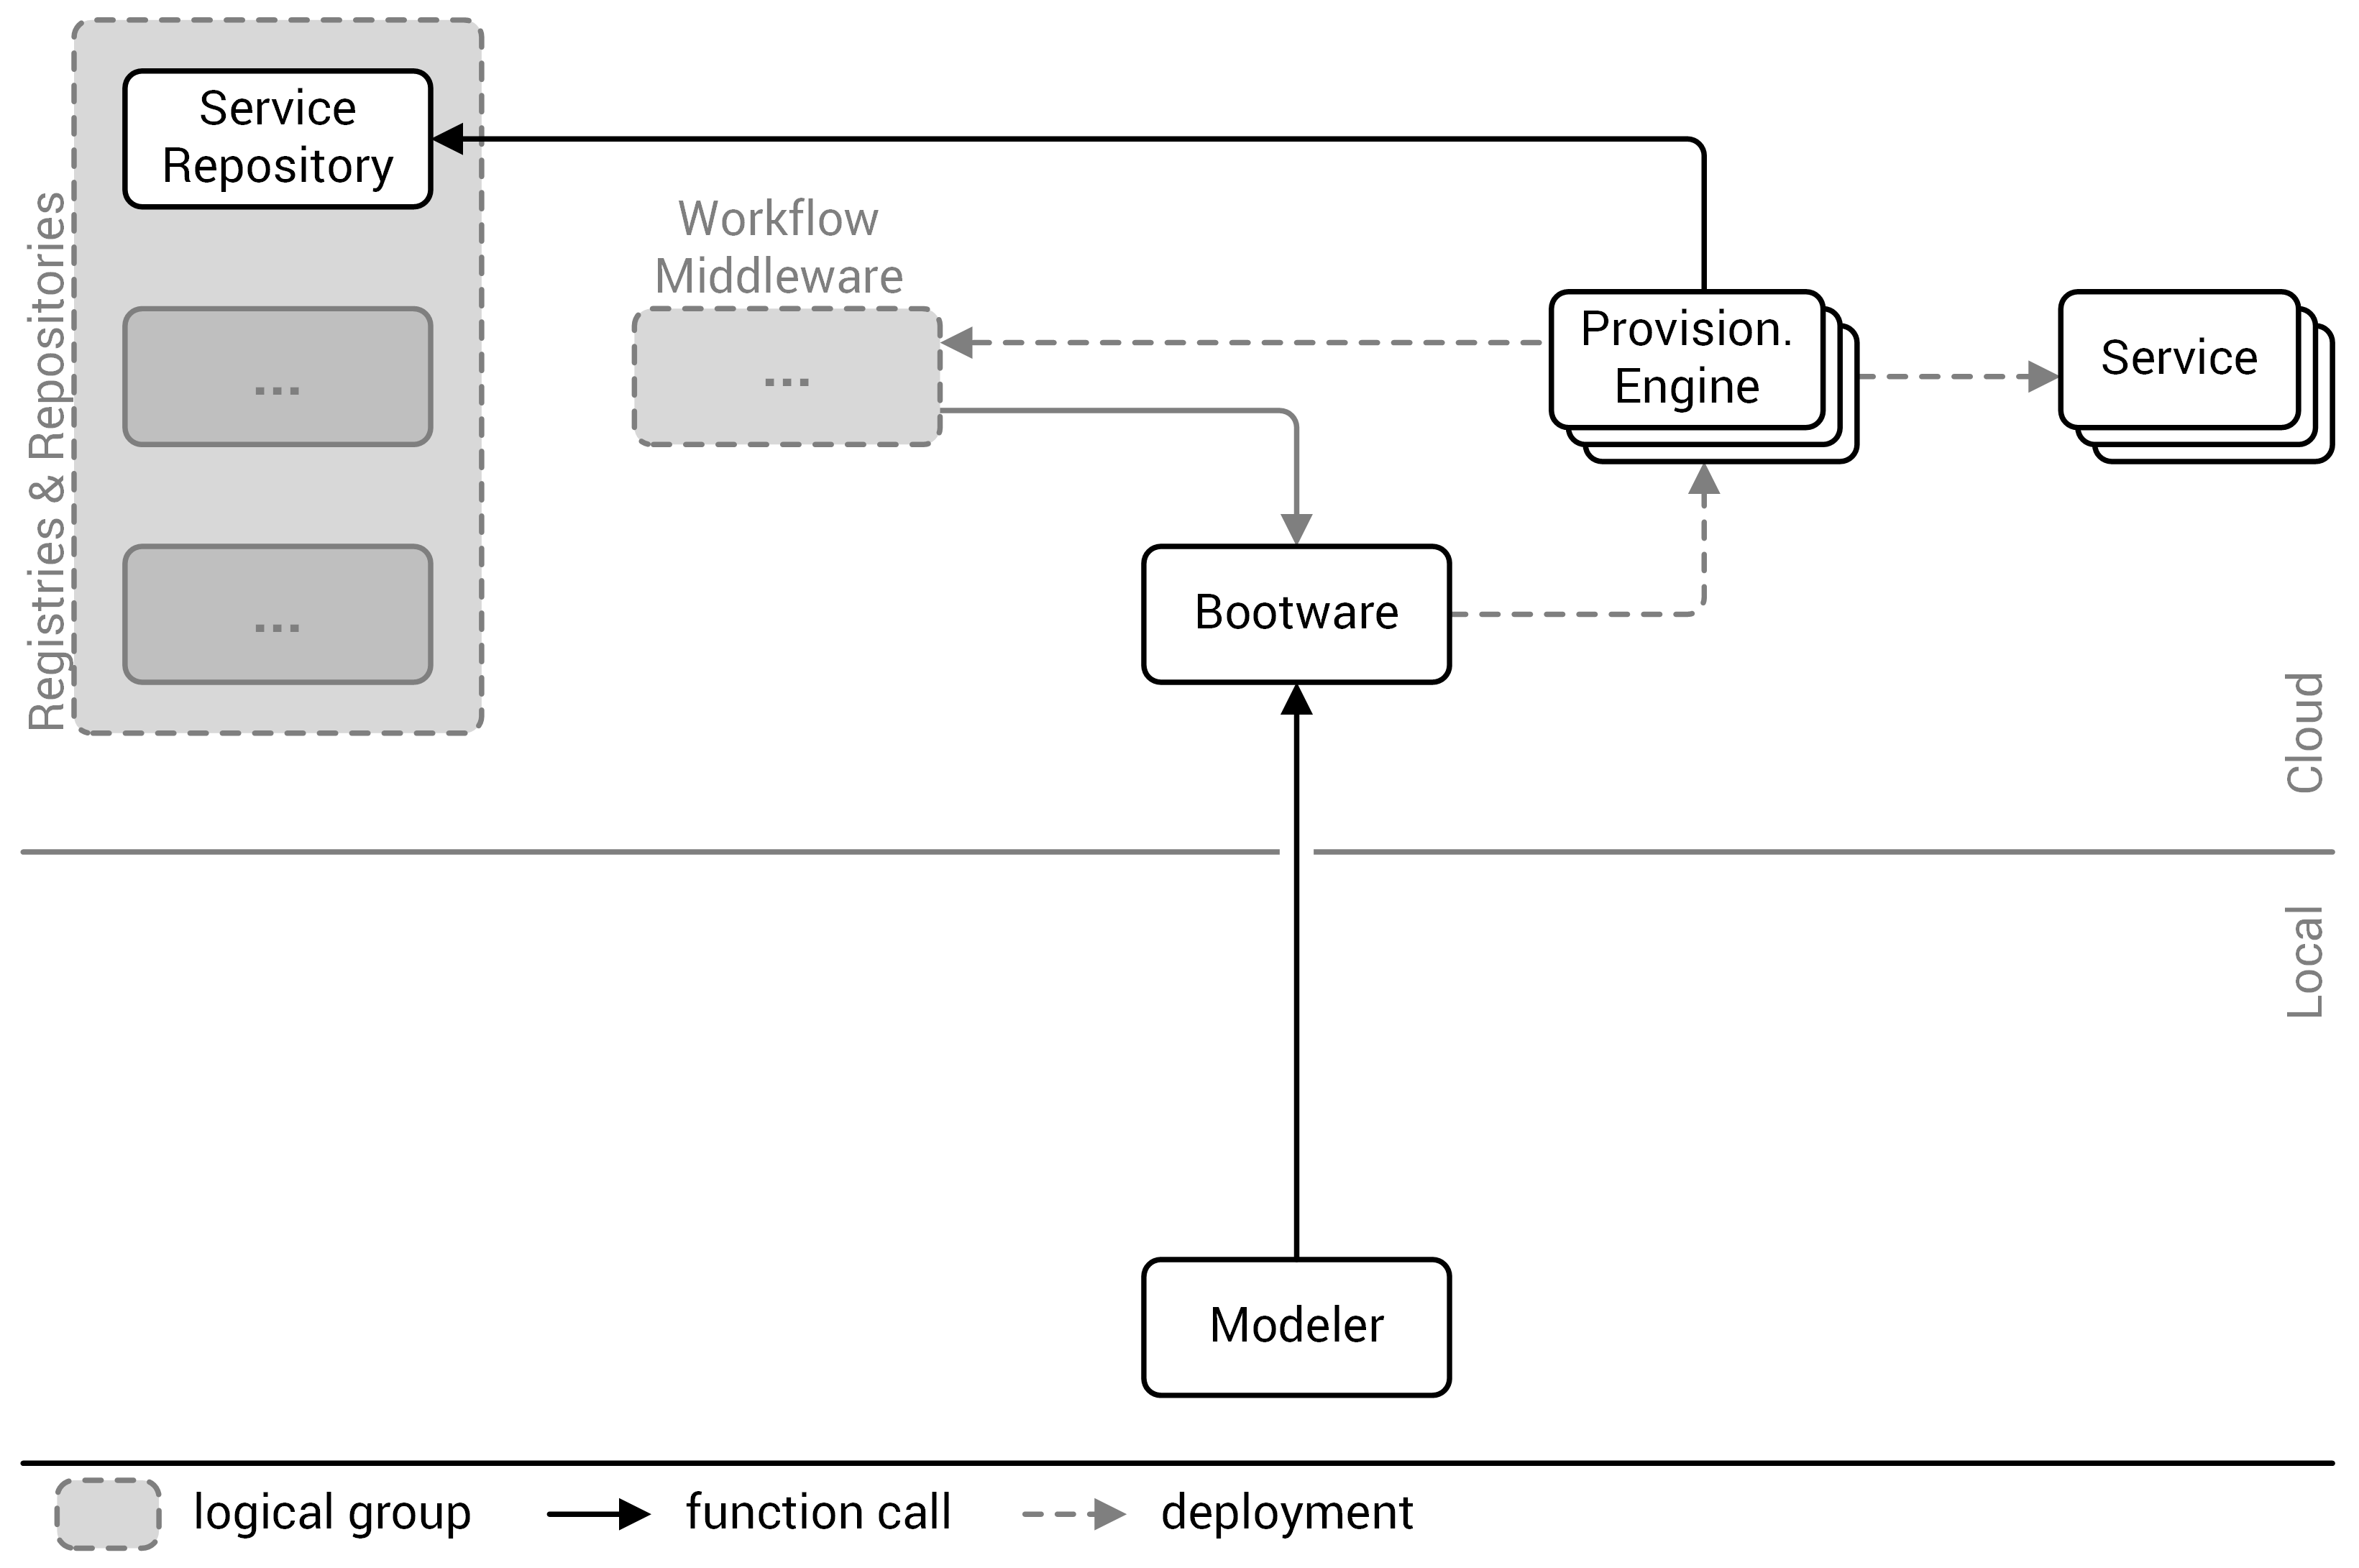
\includegraphics[resolution=600]{design/assets/simple_remote}
	\caption{Simplified overview of the single remote component architecture}
	\label{image:single_remote}
\end{figure}

The next obvious choice is to put the single bootware component into a remote environment, where the disadvantages of local to remote communication would disappear.
However, this creates new problems.

Since there aren't any additional components in this scenario that could manage the life-cycle of the remote bootware, the user would have to manage it by hand, which leads to two possibilities.
Either the user provisions the bootware once in some cloud environment and then keep this one instance running or she provision it once she needs it and deprovisions it when she is done.

In the first case the user would only have to provision the bootware once, but this creates a new problem: The user doesn't know where exactly to put the bootware component.
Since one requirement is that multiple cloud environments should be supported, it's possible that the bootware component is not located anywhere near the cloud environment where it should provision further components.
The communication problem of the single local bootware component can still occur in these cases.

Another problem is that the bootware would be running all the time, even if the user doesn't need it, which would increase costs.
This problem could be reduces if this bootware instance is shared with others to assure a more balanced load.
But then the user would have to manage some sort of load balancing and the bootware component would have to support multi-tenancy or be stateless to be able to cope with potential high usage spikes.
This would further complicate the design and implementation of the bootware component and possibly increase the running costs.

In the second case the user would provision the bootware whenever she needs it.Now the user would be able to pick a cloud environment that is close to the other components that she plans to provision later.
This eliminates the two major problems of the first case but increases the effort that the user has to put into a task that she shouldn't have to do in the first place.
Life-cycle management of the bootware should be automated completely and hidden away from the user.
Therefor, this scenario is not appropriate for our case.

\subsubsection{2-Tier Architecture}
\label{design:division:2tier}

\begin{figure}[!htbp]
	\centering
	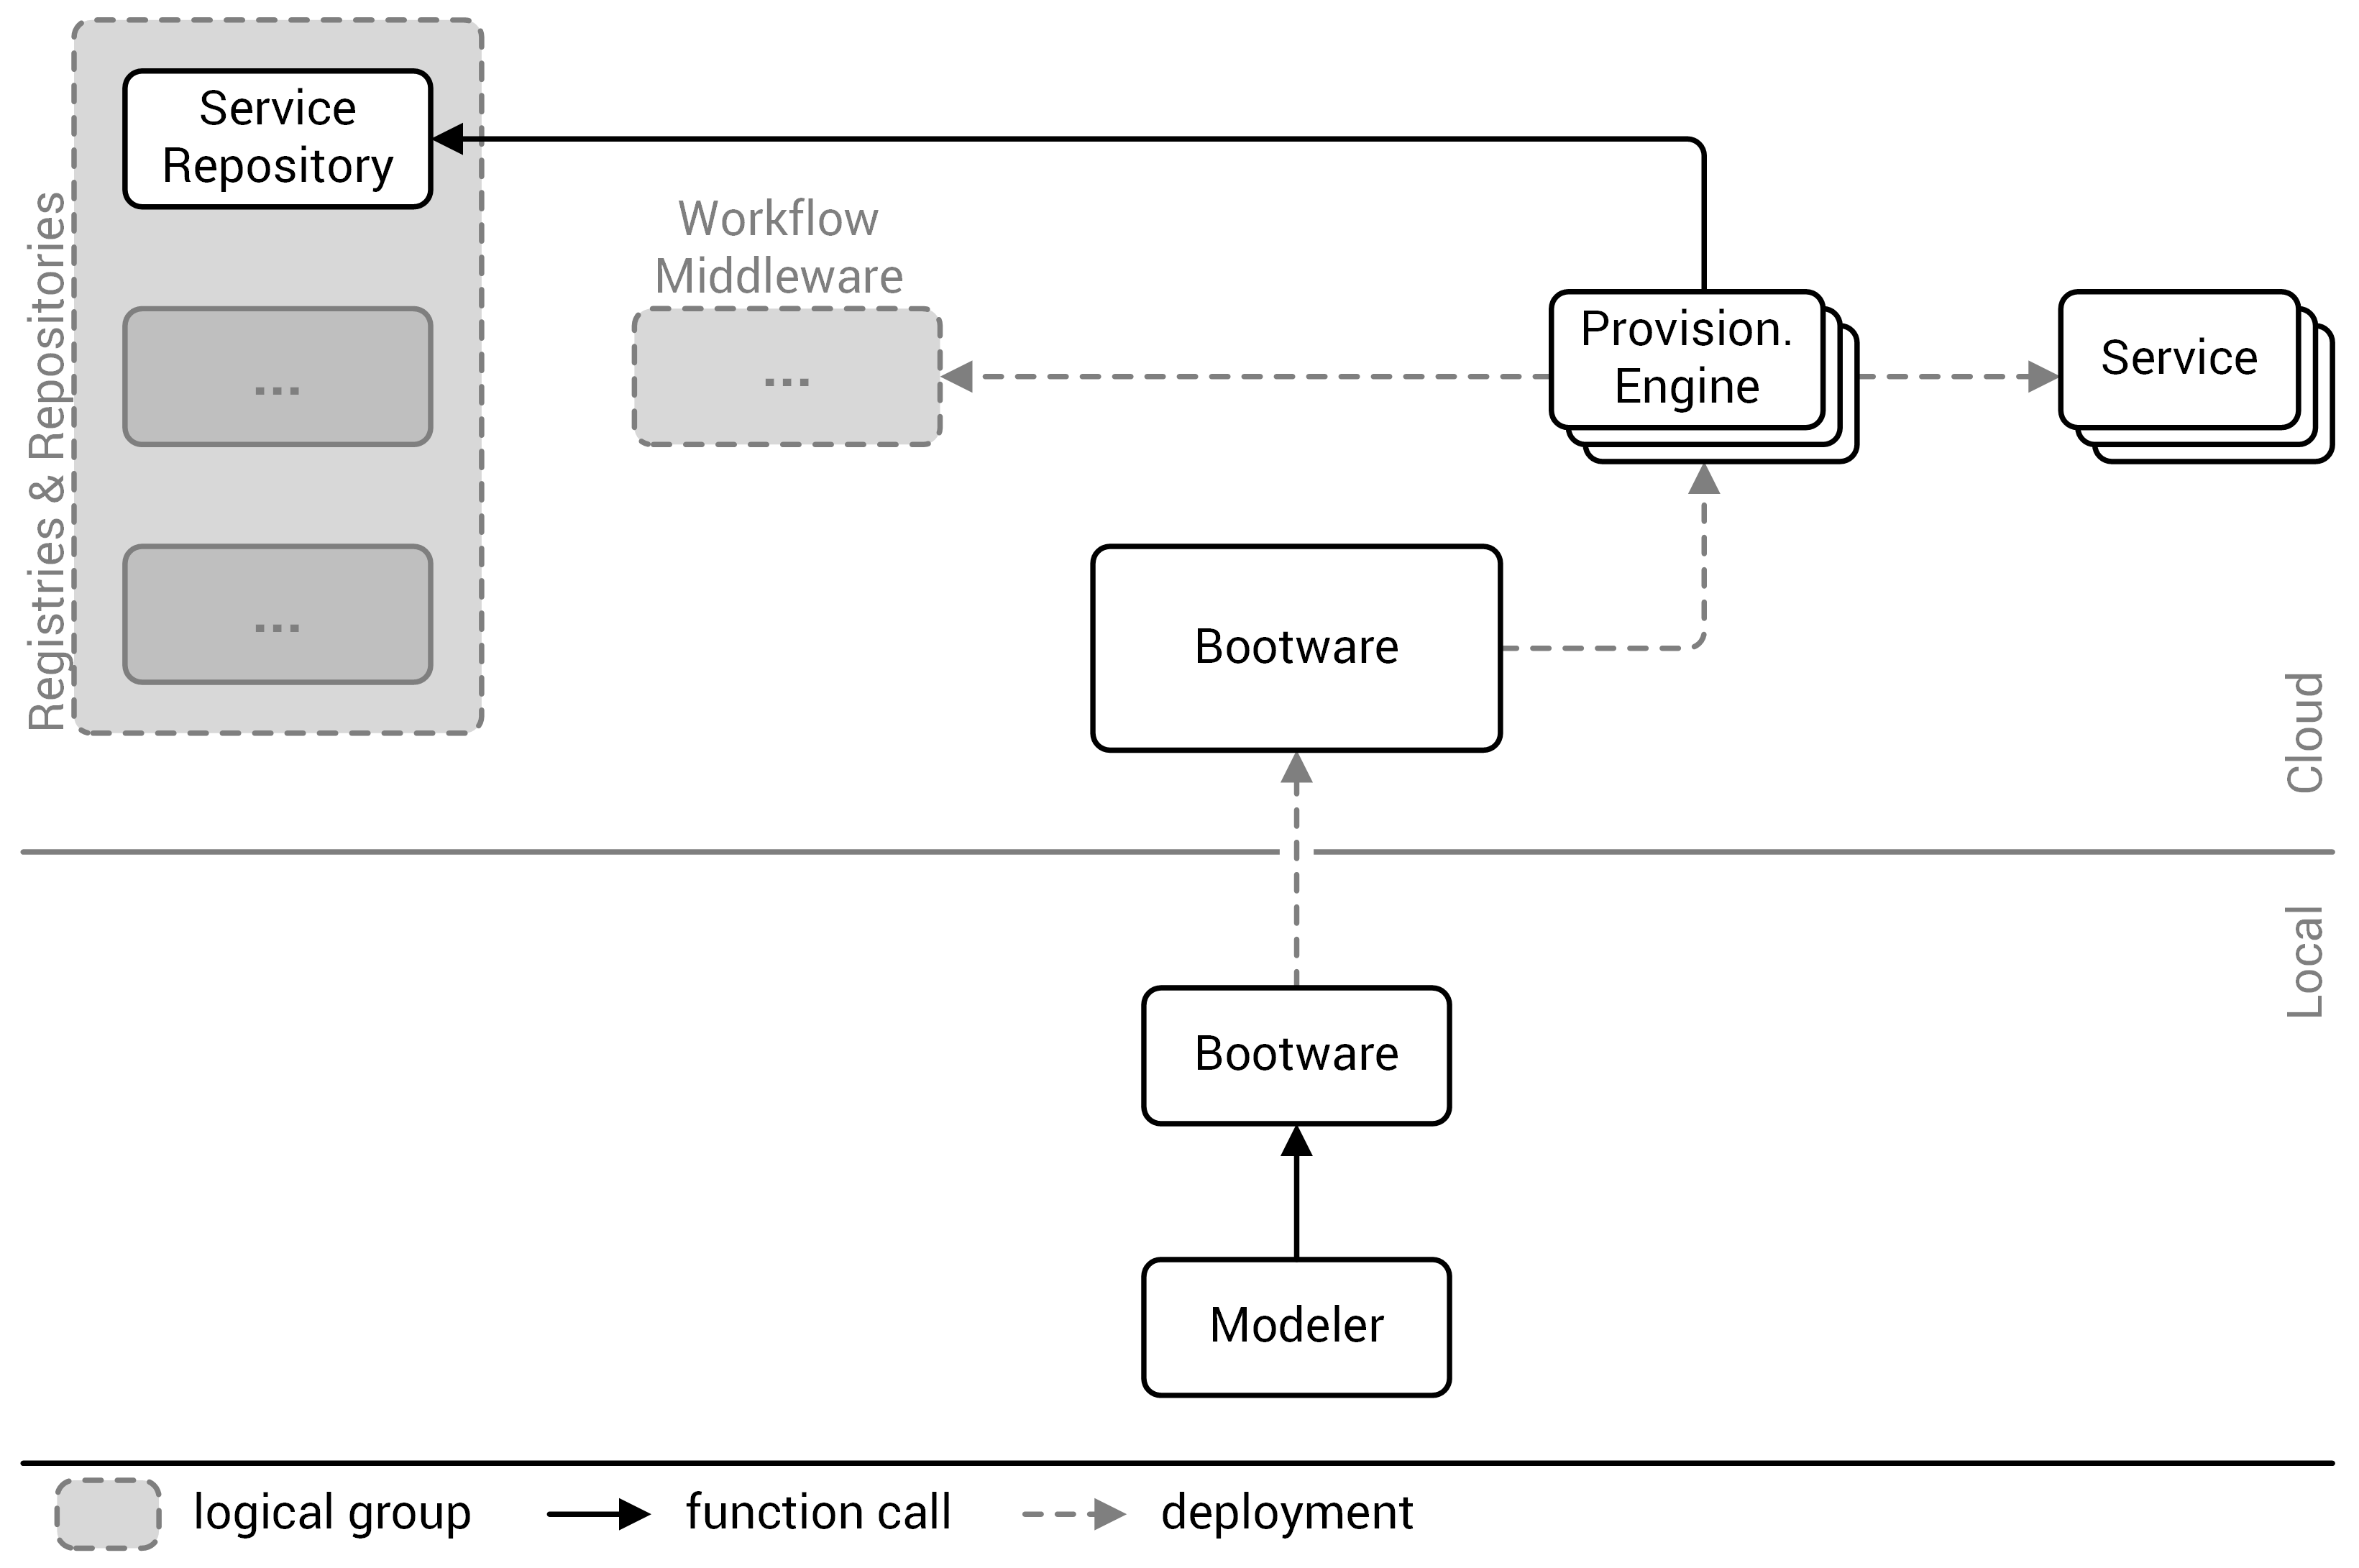
\includegraphics[resolution=600]{design/assets/simple_2_tier}
	\caption{Simplified overview of the 2-tier architecture}
	\label{image:2_tier}
\end{figure}

Next, we take a look at a 2-tier architecture, where the bootware is divided into two components.
On the local side we have a small and simple component which has mainly one function: To provision the larger second part of the bootware in a remote environment near to the environment, where other components will be provisioned later.

This eliminates the problems of a single local or remote bootware component.
The user no longer has to be involved in the management of the remote bootware since the local bootware handles all that.
Since we provision the remote bootware on demand we now also can position the remote component close to other remote components to minimize local/remote communication and the problems resulting of it.
We can now keep the local part as simple as possible and make the remote part as complicated as it has to be and since we provision the remote bootware only for one user we don't have to worry about multi-tenancy.

But we also introduce new problems.
For one, we now have duplicate functionality between the two components.
Both components have to know how to provision a component into multiple cloud environments.
The local component has to be able to put its remote counterpart into any cloud environment.
The remote component has to be able to provision other components into the same environment in which it runs (ideally, to minimize costs).
Since itself can be located in any cloud environment, it has to be able to do this in any cloud environment.
Independent from this, it has to be able to provision to any environment that the user/service package chooses.
But this problem can be solved by using a plugin architecture, which allows both components to use the same plugins.
We discuss plugins in detail in \autoref{design:extensibility}.

\textcolor{red}{A second problem which we can't avoid but can solve is the communication which is now necessary between the different parts of the bootware.
More on this in \autoref{design:communication}}

\subsubsection{Cloning}

\begin{figure}[!htbp]
	\centering
	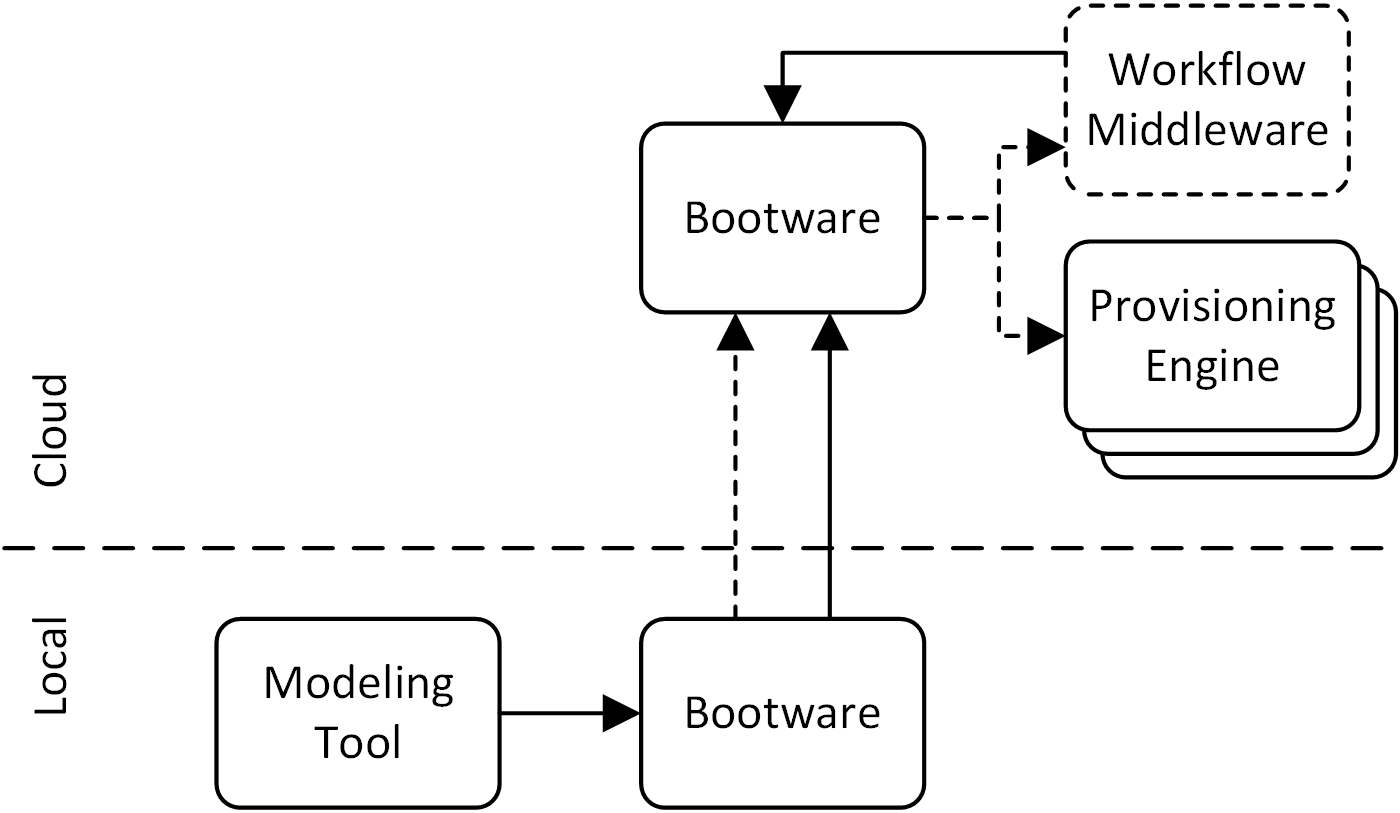
\includegraphics[resolution=600]{design/assets/simple_clone}
	\caption{Simplified overview of the cloned component architecture}
	\label{image:clone}
\end{figure}

This architecture can be seen as an alternative form of the 2-tier architecture described in \autoref{design:division:2tier}.
In this case there are also two parts working together and the remote part does most of the work.
However, the local and the remote components are identical.
Instead of provisioning a bigger component in a remote environment, the local component clones itself.
Compared to the 2-tier architecture described before, this has the advantage that only one component has to be designed and implemented and that function duplication is not an issue.
The disadvantage would be that the local bootware would be exactly as complex as the remote bootware and would contain unnecessary functionality (e.g. a web service interface).
However, since we want to keep the whole bootware, including the remote part, fairly lightweight, it's highly unlikely that the complexity of the remote bootware will reach such heights that it could not be run on an average local machine.
In this case, the advantage of only having to design and implement one component seems to outweigh the disadvantage of a slightly more complex local component (compared to the 2-tier variant).
Of course, this architecture makes only sense if the functionality of the two separate components in the 2-tier architecture turns out to be mostly identical.
Therefore we can't decide yet if this architecture should be used.

\subsubsection{Decision}

Of the four alternative presented here, alternative three - the 2-tier architecture - makes the most sense.
Therefore it is selected as the alternative of choice and used for further discussion.
We do however retain the option to transform it into alternative four if we discover that both components share much of same functionality, but this can only be judged at a later stage, when we know exactly how the internal functionality of the bootware will work.

\section{Extensibility}
\label{design:extensibility}

In \autoref{design:communication} we mentioned a secondary communication mechanism that would be best implemented in form of an extension to the bootware.
The requirements for the bootware also state that support for different cloud environments and provisioning engines should be achieved through means of software engineering.
These requirements are intentionally vague to allow for the selection of a fitting extension mechanism during the design process.
In this section we will take a look at different extension mechanisms for Java and pick the one that suits our needs best.

\subsection{Extension Mechanisms}

The simplest way to fulfill the extensibility requirement would be to create a set of interface and abstract classes to define the interfaces and basic functionality that are necessary to work with different cloud environments and provisioning engines.
These interfaces and abstract classes would then be implemented separately to support different scenarios and would be compiled, together with the rest of the application, into one executable.
At runtime, a suitable implementation would be selected and used to execute the specific functionality required at this time.

This extension mechanism is simple, but restricted by its static nature.
The entire executable has to be recompiled if any implementations are changed or added.
This may not be a problem if the set of possible extensions that have to be supported is limited and known at the time of implementation or if it changes rarely.
If the set of necessary extensions is unknown or changing from time to time, implementing new or changing existing extensions can get cumbersome because a new version of the whole software has to be released each time.
It would be far better if extensions could be implemented separately from the core bootware components and added and removed at will.

A more flexible architecture is needed, for example a plugin architecture.
Interfaces for the extension points still exist but the extension are no longer part of the main bootware components.
They are compiled separately into plugins that can be loaded into the main bootware components on the fly.
There are several possibilities to realize such an architecture.

It is certainly possible to implement a plugin framework from scratch.
An advantage of this approach would be that the design of the plugin architecture could be tailored to our use case and would be as simple or complex as needed.
But there are also several disadvantages.
For one, we would reinvent the wheel because multiple such frameworks already exist.
It would also shift resources away from the actual goal of this diploma thesis, which is designing the bootware.
Furthermore, it would require a deep understanding of the language used for the implementation (in this case Java), which is not necessarily given.
Therefore, it seems more reasonable to use one of the already existing plugin frameworks.
Which one exactly will be determined later in \autoref{implementation:selecting:pluginframeworks}.

\subsection{Plugin Repository}
\label{design:pluginrepository}

Now that we have introduced plugins we face new problems.
\autoref{image:plugins} shows the current architecture, where both bootware components use their own plugins.
If a plugin is added or updated, the user has to manually copy this plugin to the right folder of one or both of the bootware components.
Furthermore, if both components use the same plugins, which they will (for example plugins for different cloud providers), we will have duplicate plugins scattered around.
This is inefficient, probably annoying for the user and can cause errors if plugins get out of sync.

\begin{figure}[!htbp]
	\centering
	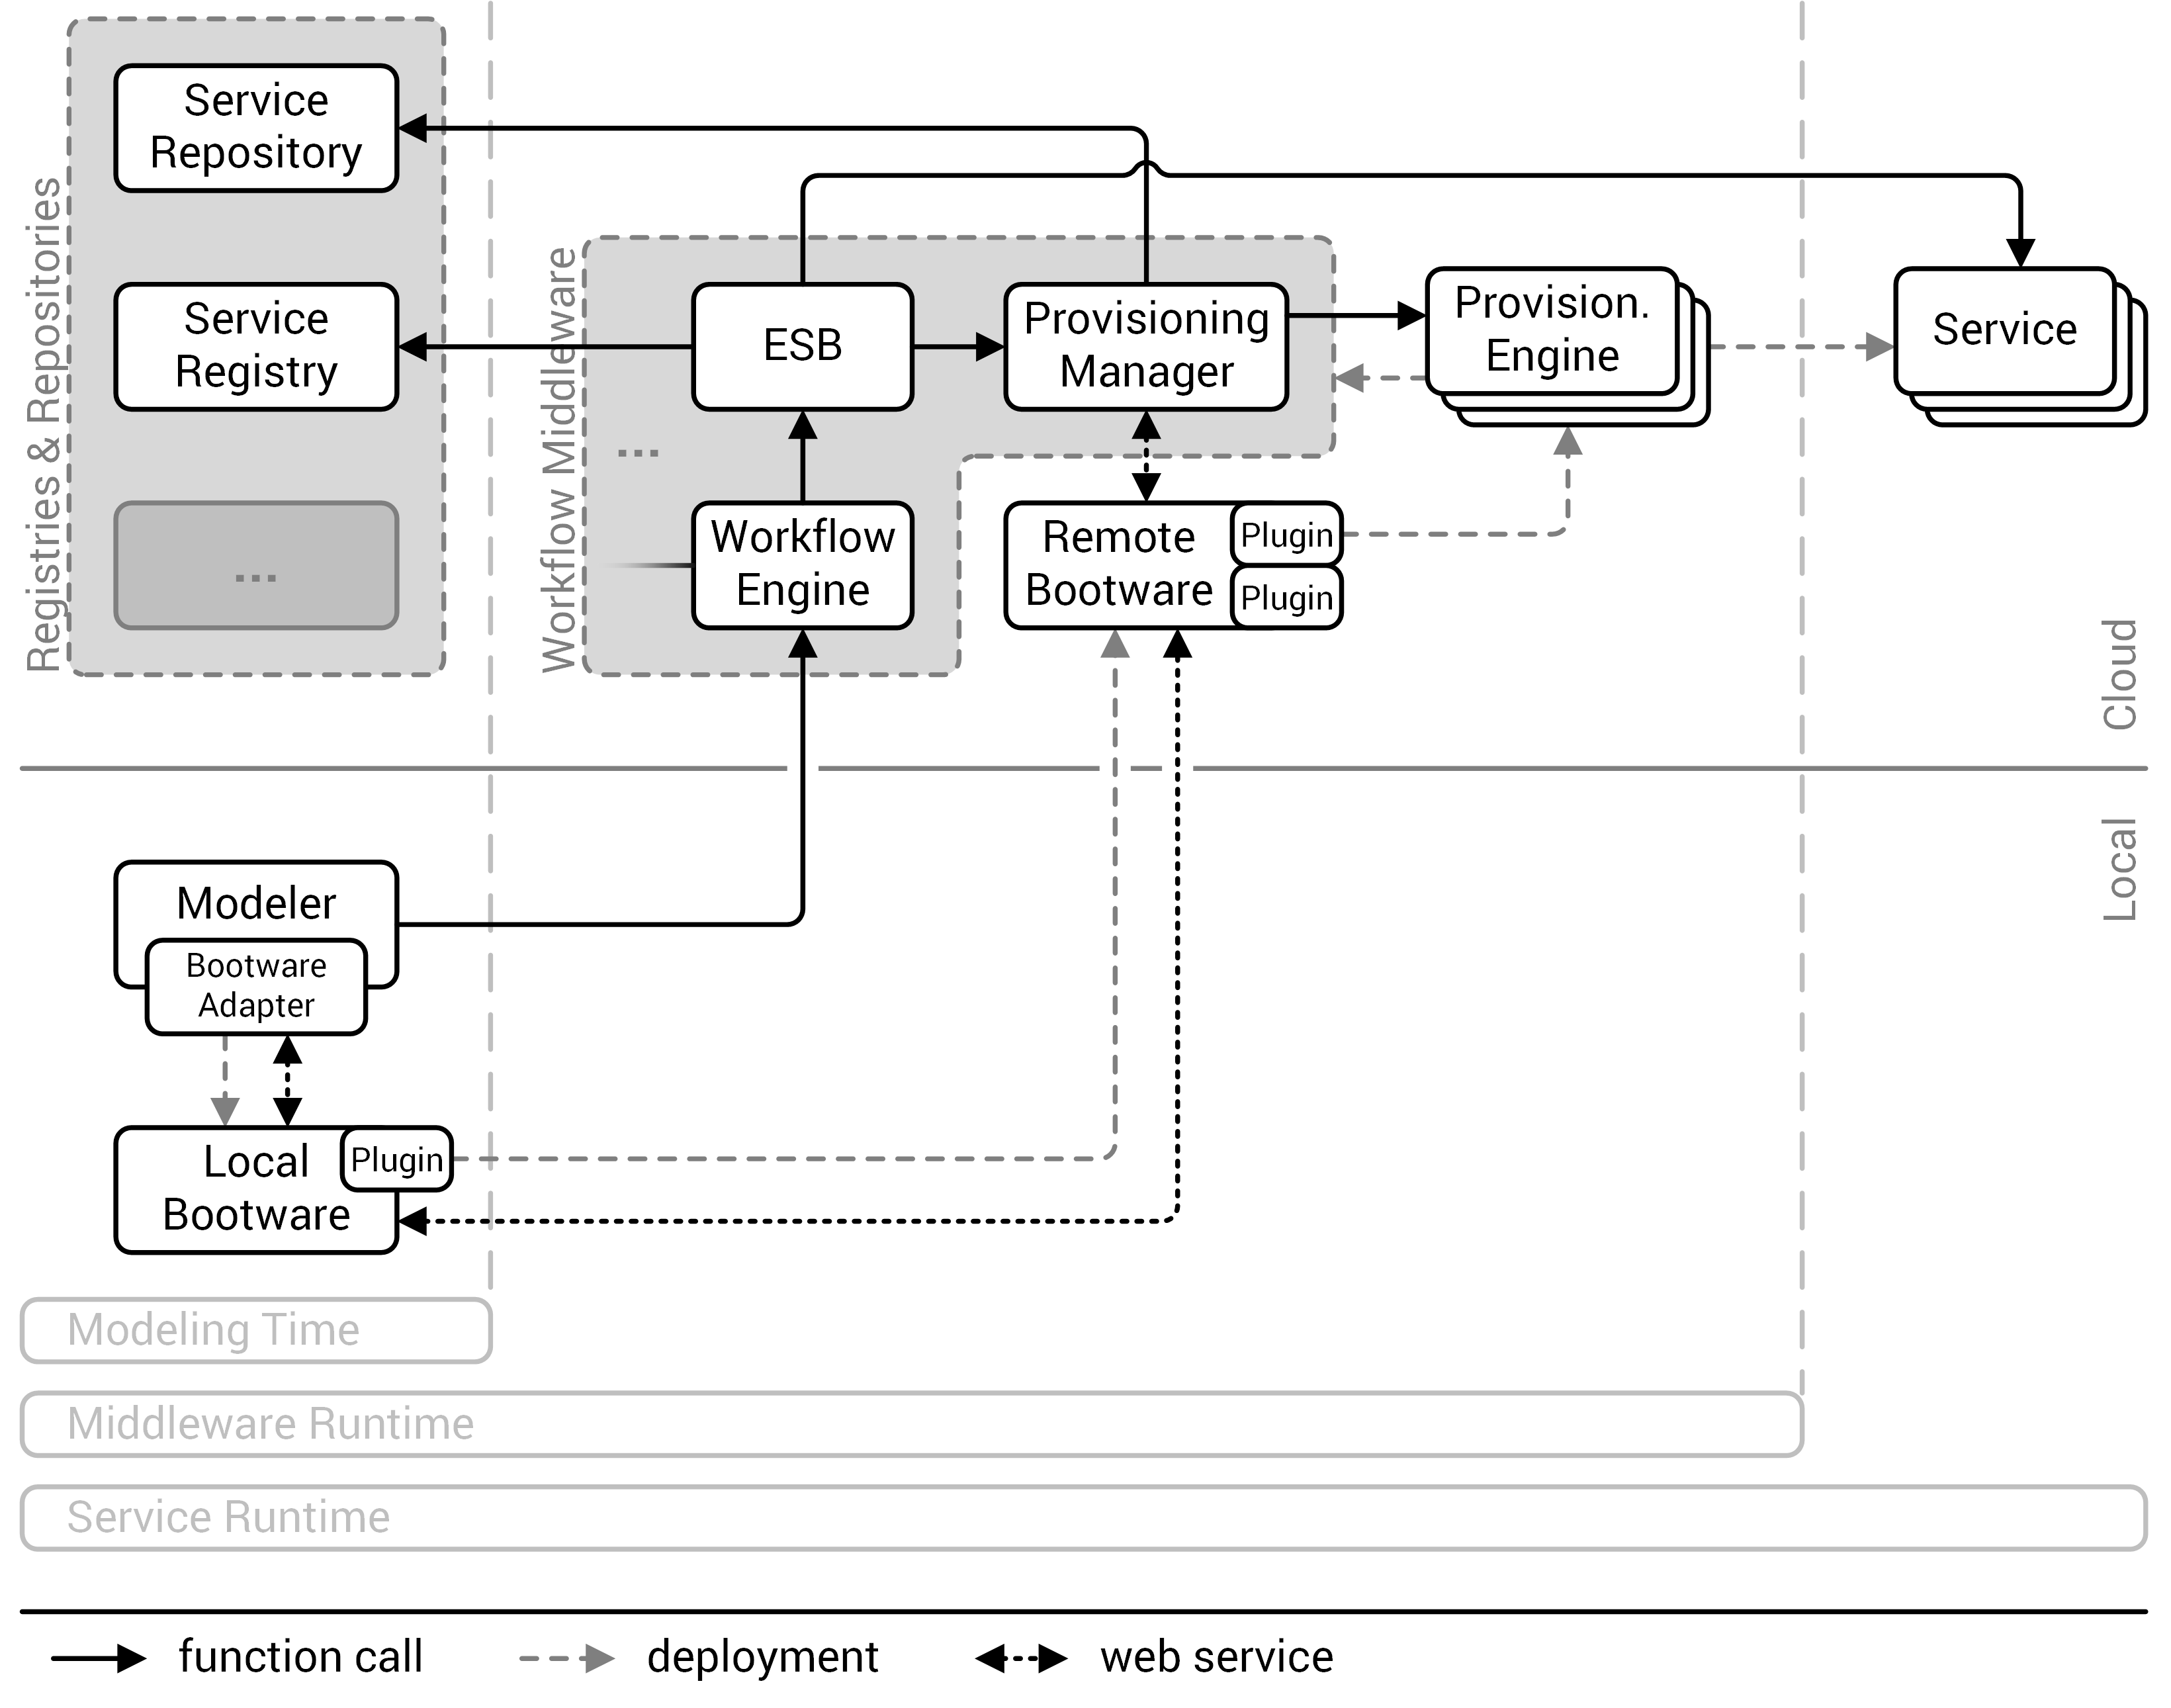
\includegraphics[resolution=600]{design/assets/plugins}
	\caption{Simplified overview of the 2-tier architecture with plugins.}
	\label{image:plugins}
\end{figure}

To remedy this situation we introduce a central plugin repository, as shown in \autoref{image:plugin_repository}.
This repository holds all plugins of both components so it eliminates duplicate plugins.
If plugins are added or modified it has only to be done in one place.
Plugin synchronization can happen automatically when the bootware components start, so that the user is no longer involved in plugin management.
The repository also enables easy plugin sharing, which was cumbersome earlier.
While a central plugin repository is a sensible addition to the proposed bootware architecture, its design and implementation are out of scope of this diploma thesis.
This work is left for the future and the plugin repository will not be mentioned in any other figures apart from \autoref{image:plugin_repository}.

\begin{figure}[!htbp]
	\centering
	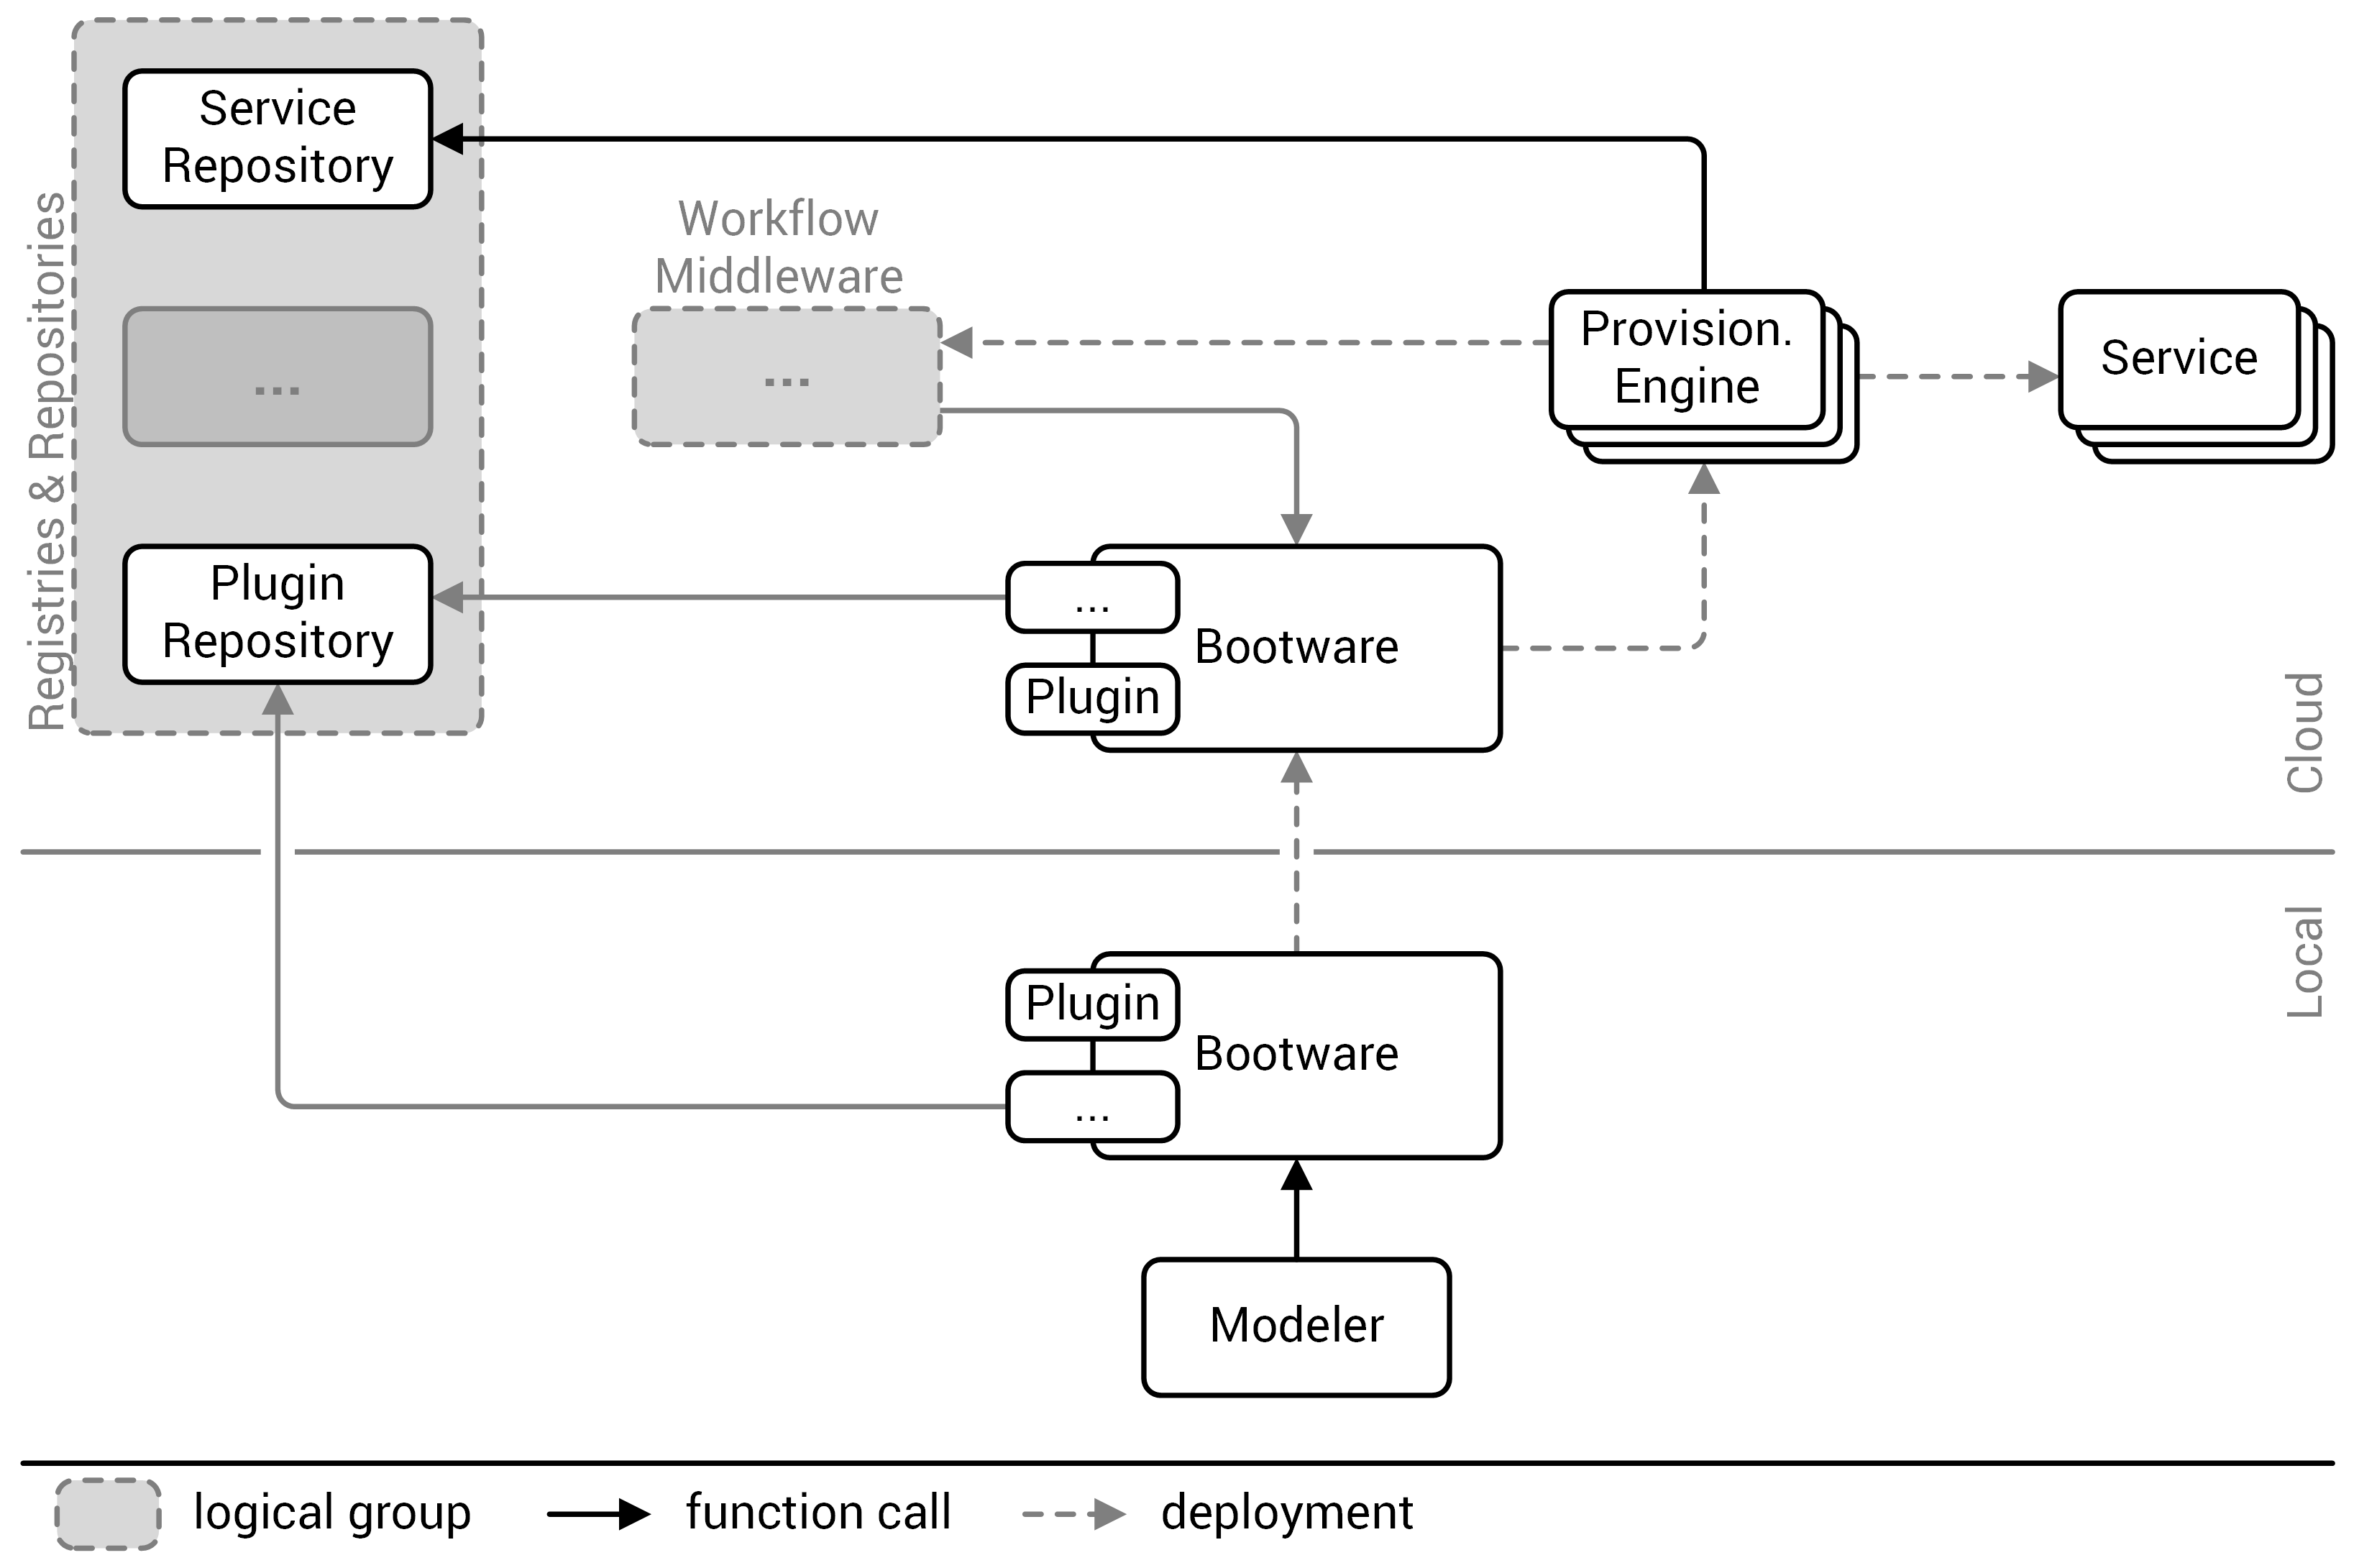
\includegraphics[resolution=600]{design/assets/plugin_repository}
	\caption{Simplified overview of the 2-tier architecture with a plugin repository.}
	\label{image:plugin_repository}
\end{figure}

\section{External Communication}
\label{design:communication}

In \autoref{design:modeler_integration} we established that a bootware plugin in the modeler has to call the local bootware.
From \autoref{design:division} we also know that both the local bootware and the provisioning manager have to call the remote bootware.
We now have to decide, how this external communication with the bootware will work.
There are several factors that impact this decision.
Communication between the components should be as simple as possible, but has to support some critical features.
To keep it simple, it would make sense to use the same communication mechanism for communication between the bootware components as well as with other external components, like the provisioning manager and the modeler plugin.

Since the provisioning processes kicked off by the bootware can potentially take a long time to finish (in the range of minutes to hours), asynchronous communication should be used between the components to avoid timeouts and blocking resources.
For the same reason, there should be some mechanism to get feedback on the current status during a long running provisioning process.

The communication with the bootware components will contain sensitive data, for example login information for cloud providers.
This information has to be provided from the outside and should be transported securely to prevent malicious or fraudulent attacks.
The selected communication method therefore has to support some sort of security mechanism, ideally end-to-end encryption.
While these security mechanisms will not be used in this thesis due to time constraints, selecting the right communication method is still critical for future development.

Java provides a package for \nom{Remote Method Invocation}{RMI}\footnote{\url{http://docs.oracle.com/javase/7/docs/api/java/rmi/package-summary.html\#package_description}}, which allows objects in one Java VM to invoke methods on objects in another Java VM.
But since RMI is limited to Java and we might want to communicate with the bootware from a component written in another programming language, RMI doesn't seem like a good fit.
For communication between programs written in different languages we could use the \nom{Common Object Request Broker Architecture}{CORBA}, a standard defined by the \nom{Object Management Group}{OMG}.
It supports mappings for common programming languages, like Java, C++, Python, and others.
CORBA also supports asynchronous method invocation via callbacks~\autocite{corba:async} and transport layer encryption and other security features~\autocite{corba:security}.

As a second alternative, we could communicate with messages by using message-oriented middleware.
As explained earlier in \autoref{fundamentals:service}, it supports communication between different components using adapters and channels.
Asynchronous communication is supported by using message queues for temporary storage.
The middleware can also provide additional persistent storage and backups for high availability~\autocite{mom}.
It may also support security features like encryption.
Another alternative are web services via \nom{Simple Object Access Protocol}{SOAP} or \nom{Representational State Transfer}{REST}.
Like CORBA, web services also support asynchronous invocation, as well as security mechanisms~\autocite{ws:security}.

\begin{figure}[!htbp]
	\centering
	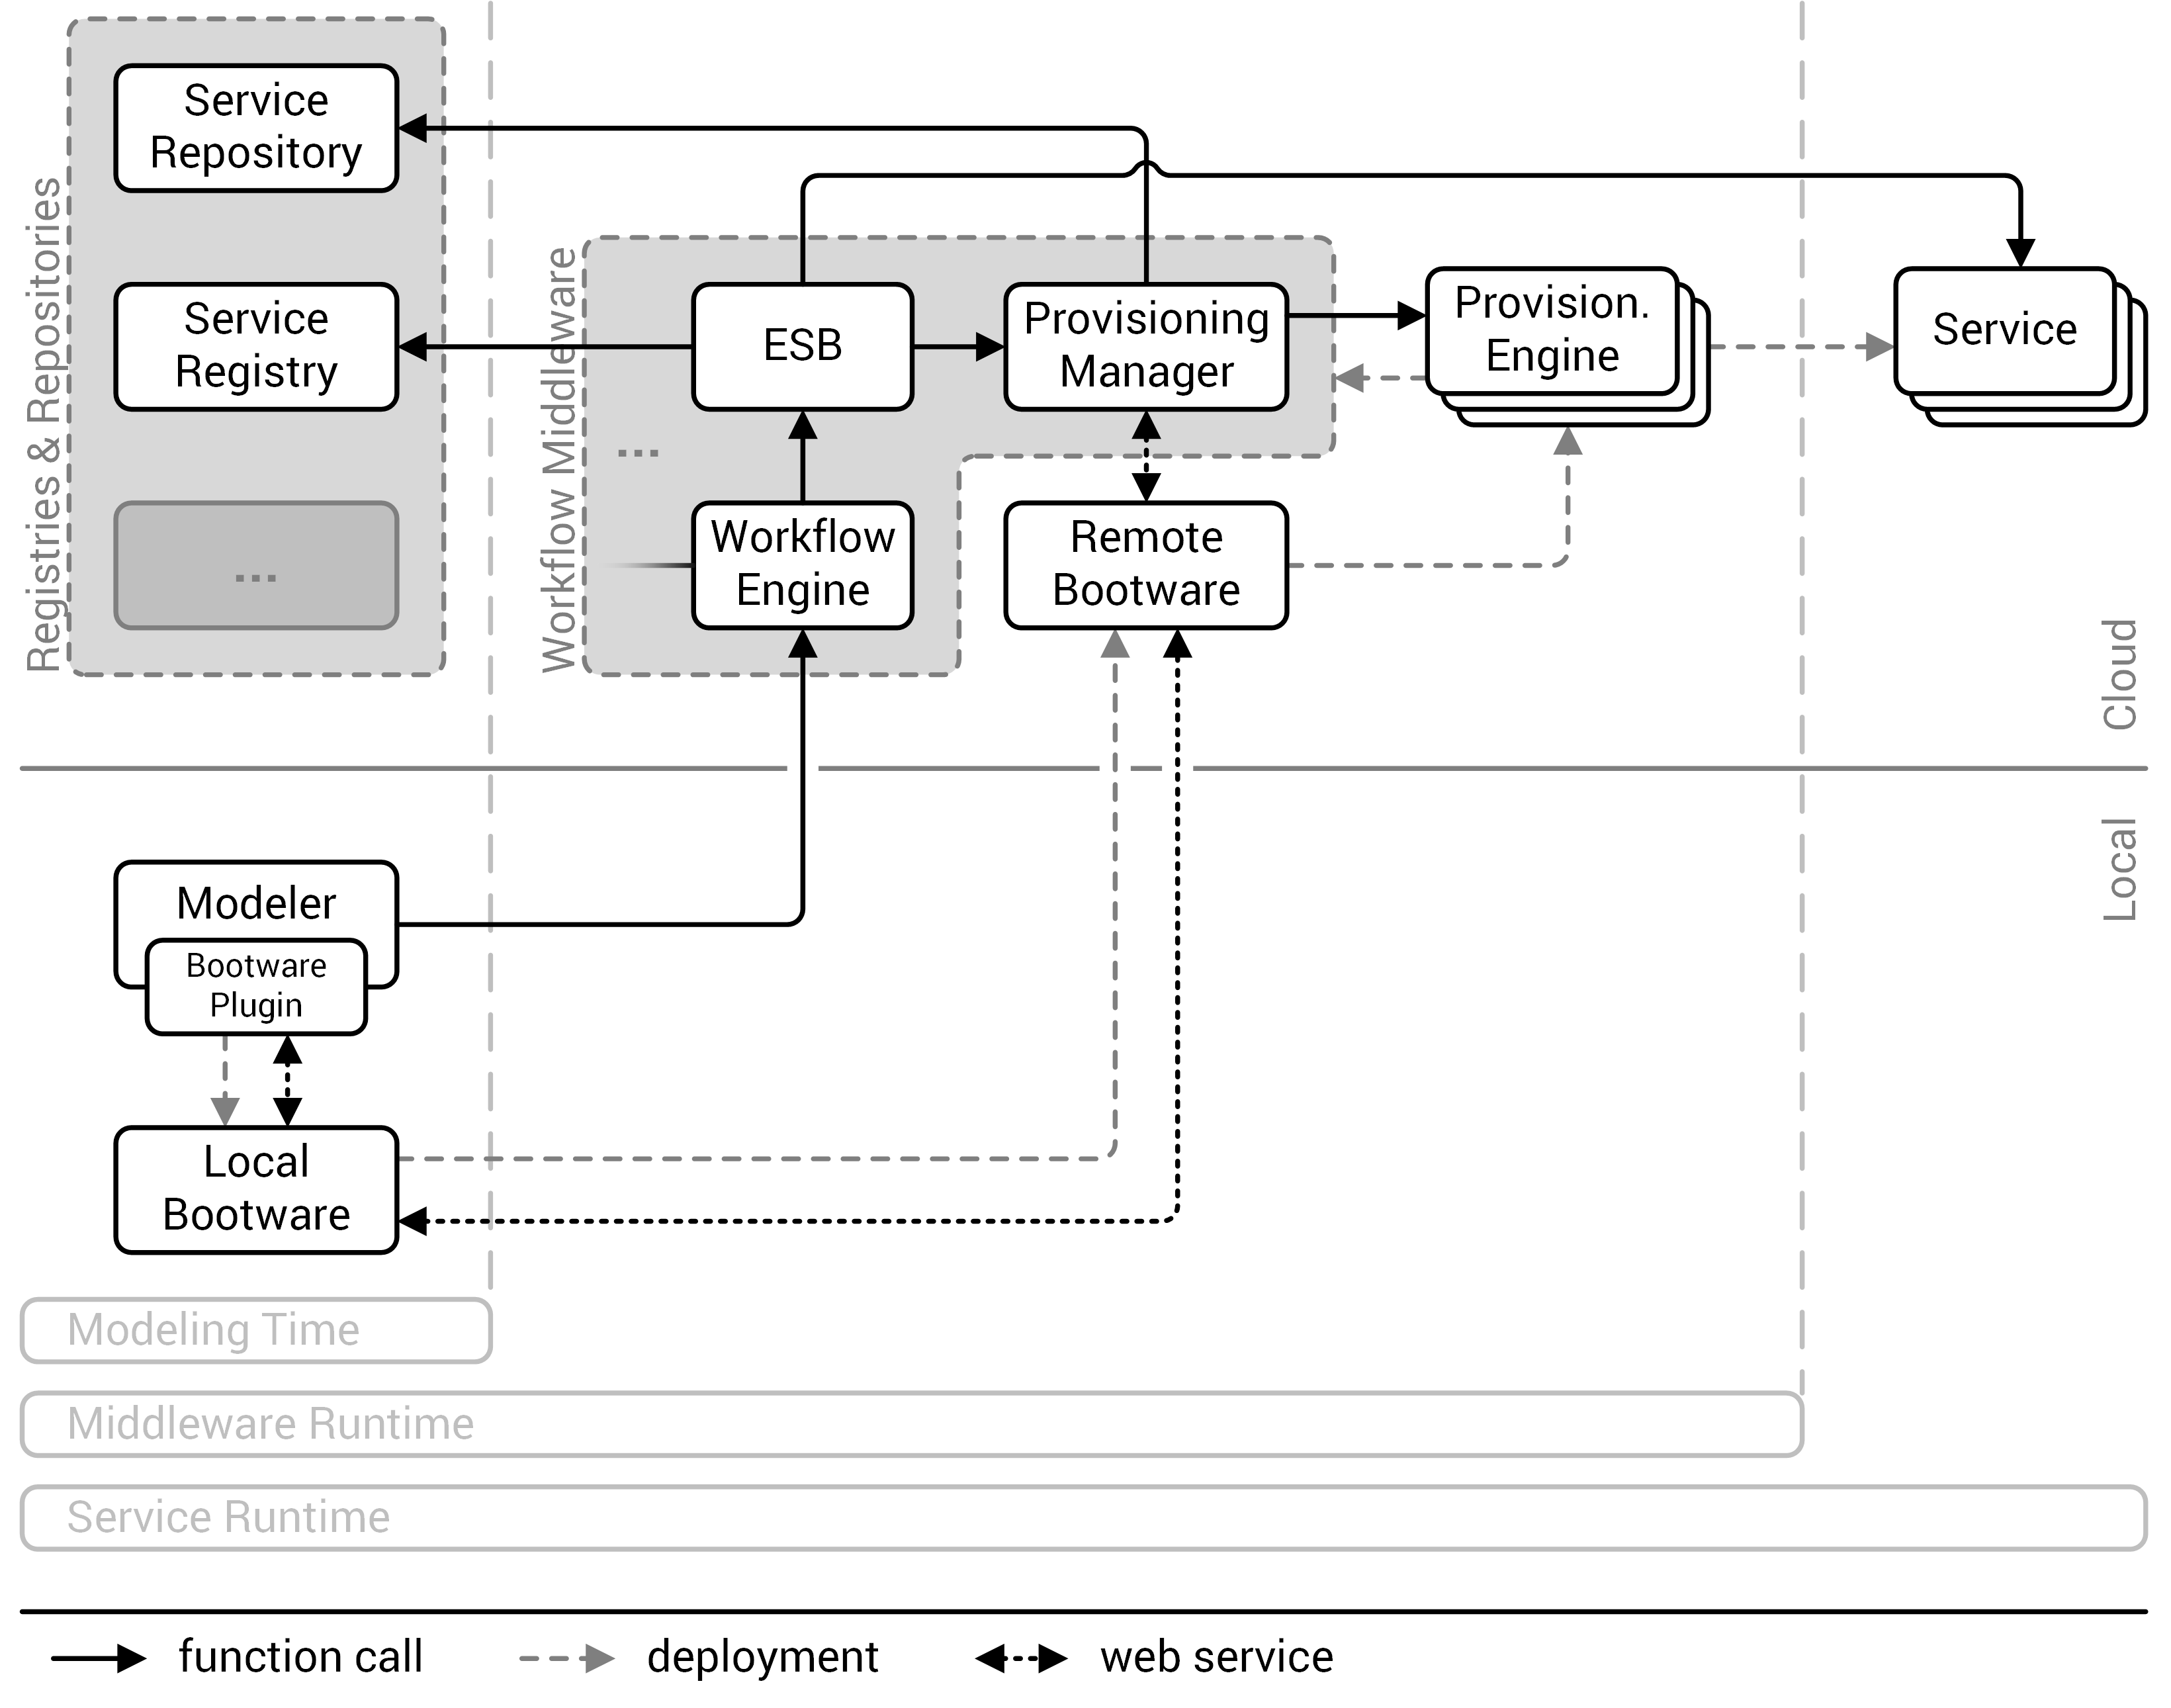
\includegraphics[resolution=600]{design/assets/webservice}
	\caption{Simplified overview of the 2-tier architecture with asynchronous web service communication}
	\label{image:webservice}
\end{figure}

Since the whole SimTech SWfMS already uses SOAP based web services, it would make sense to also use SOAP based web services as external communication mechanism for the bootware.
The technology and knowledge is already in place and introducing a second mechanism like CORBA would unnecessarily increase the complexity of the project, especially since CORBA doesn't offer any significant advantages over SOAP based web services.
\autoref{image:webservice} shows the addition of asynchronous web service call and return communication between the modeler bootware plugin and the local bootware, and between the remote bootware and the local bootware, as well as the provisioning manager.

With asynchronous communication, long running provisioning processes won't pose a problem.
We do however still need information during those long running processes to give the user some feedback.
This can't be accomplished by the simple web service request/response pattern.
For this, a secondary communication mechanism which supports sending multiple feedback messages has to be used.

\begin{figure}[!htbp]
	\centering
	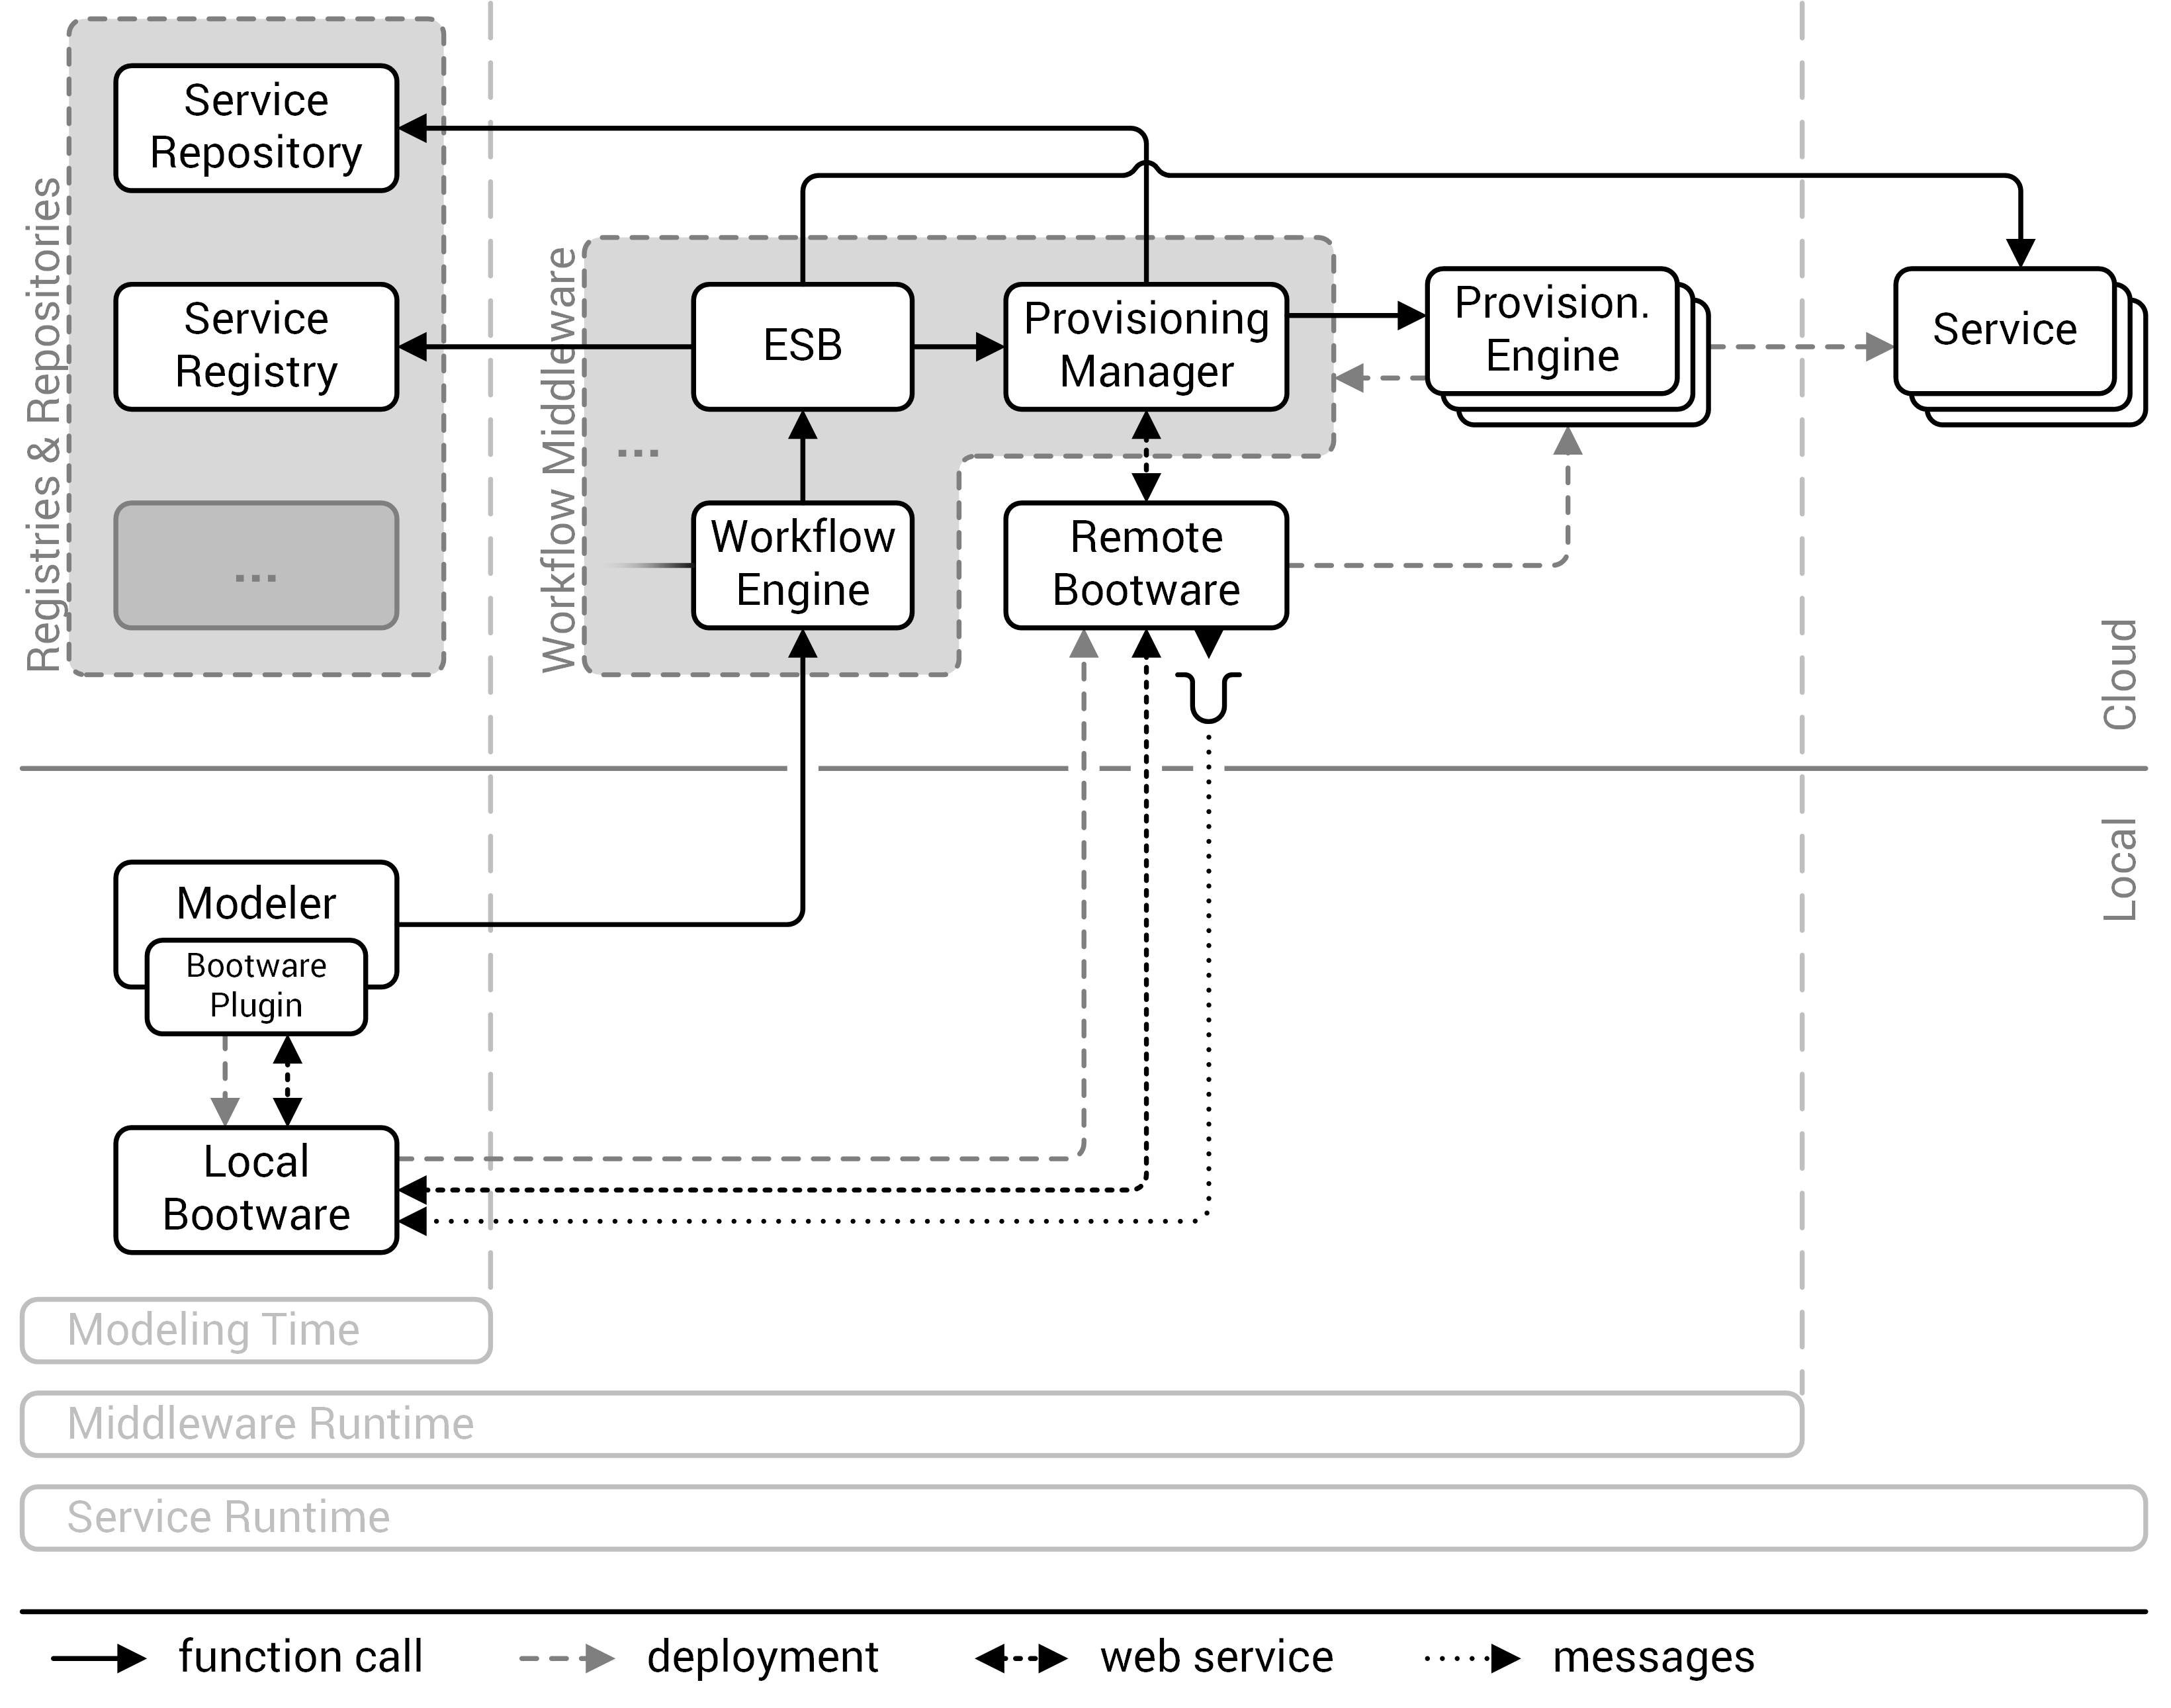
\includegraphics[resolution=600]{design/assets/message_queue}
	\caption{Simplified overview of the 2-tier architecture with asynchronous web service and messaging queue communication}
	\label{image:message_queue}
\end{figure}

This secondary communication channel could take any form, but a natural choice for publishing the intermediary state of the bootware would be a message queue system.
In this case, the remote bootware pushes messages to a message queue to which the local bootware (and other components if needs be) can subscribe to receive future messages.
\autoref{image:message_queue} shows the proposed architecture with an additional (and optional) message queue that allows the local bootware or other components to listen to status updates from the remote bootware.
Since it is not necessary for the successful use of the bootware, it would make sense to implement this secondary communication mechanism as an extension to the bootware.
This extension would not be part of the core bootware, but rather an additional component that could be used when needed.
This would allow us to add arbitrary communication extensions to the bootware depending on future needs.
How this can be done will be discussed in the next section.

\section{Internal Communication}
\label{design:internalcomm}

We also have to consider internal communication between the bootware core and plugins, and possibly also in between plugins.
Ideally, every plugin will be able to react to events from the bootware.
These events could be triggered by the bootware core or by any plugin, but plugins should be completely independent from each other.
Since a plugin does not know about other plugins, it can not listen for events at other plugins directly.
The only known constant to a plugin is the bootware core.
Therefore we need a communication mechanism which allows for loosely coupled communication between the bootware core and the plugins, where plugins can register their interest for certain events with the core and also publish their own events to the core for other plugins to consume.
This essentially describes the publish-subscribe pattern~\autocite{pubsub}.

\subsection{Publish Subscribe Pattern}

The \nom{publish-subscribe pattern}{PubSub} is a messaging pattern that consists of three types of participant: An event bus (or message broker), publishers, and subscribers.
The event bus sits at the center of the communication.
It receives messages from publishers and distributes them to all subscribers that have voiced their interest in messages of a certain type by subscribing at the event bus~\autocite{pubsub}.
Using this pattern, we would create an event bus at the bootware core and plugins, as well as other parts of the core, could subscribe at this event bus and also publish messages through this event bus.

\begin{figure}[!htbp]
	\centering
	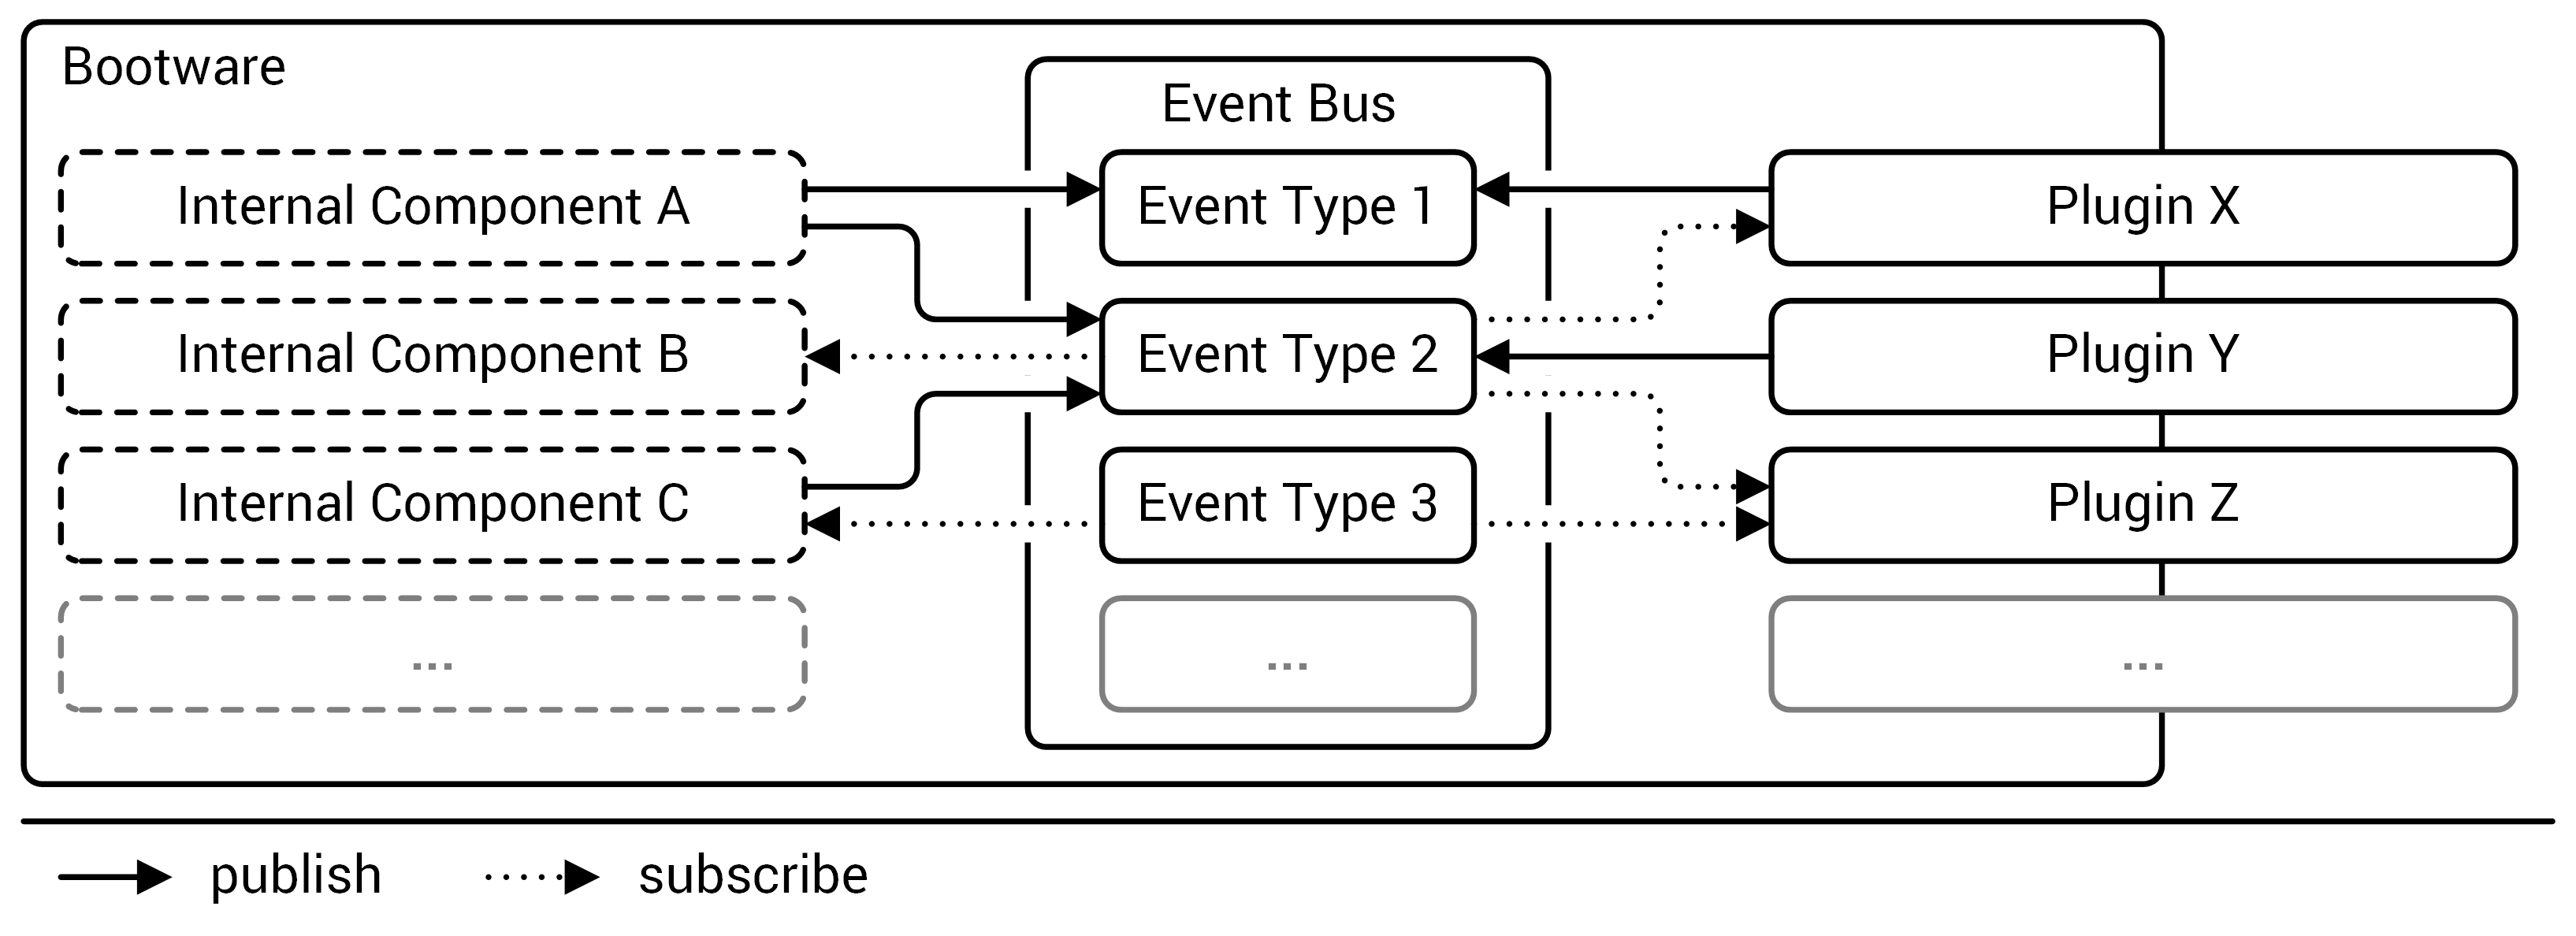
\includegraphics[resolution=600]{design/assets/pubsub}
	\caption{Bootware internal communication with PubSub pattern.}
	\label{image:pubsub}
\end{figure}

\subsection{Event Types}

When using PubSub and events to communicate, it is usually a good idea to not only use one type of event, but many different types.
Using different kinds of event allows us to subscribe only to specific events or react differently based on the type of an event.
But what if we want to react to each event type in the same way, for example for logging purposes?
Now, many different event types complicate things more.
This is where event hierarchies become useful.
At the core of an event hierarchy is a single base event.
By extending and refining this base event, other, more specific event types can be created, which again can be used as base type for even more specific events.
This allows us to create a fine grained hierarchy of events and also enables us to subscribe to particular sub sets of this hierarchy.
This makes event handling much easier, since we can now just react to the parent event if we do not need to distinguish between different event types for a particular task.

A second mechanism to differentiate between events is some sort of severity value that each event contains.
Many events will be published in an event system, but not all of them might be of the same importance.
The majority might be of low value while a few events might be very important.
For example, for logging purposes we might not be interested in every event, but only warnings and errors.
By adding a severity attribute to the base event type, all events could be categorized in different severity groups and filtered accordingly if needed.
As we can see, we might benefit from a well thought-out event hierarchy.

\vspace*{\baselineskip}
\begingroup
	\centering
	\captionsetup{type=figure}
	\begin{description}
		\item[BaseEvent] on which all other events are based
		\begin{description}
			\item[CoreEvent] published by the bootware core
			\begin{description}
				\item[PluginManagerEvent] for loading and unloading plugins
				\begin{description}
					\item[PluginLoadEvent] could be info, success, warning, or error
					\item[PluginUnloadEvent] could be info, success, warning, or error
					\item[\ldots] ~
				\end{description}
				\item[\ldots] ~
			\end{description}
		\end{description}
		\begin{description}
			\item[PluginEvent] published by a plugin
			\begin{description}
				\item[InfrastructurePluginEvent] contains further child events defined by plugin
				\item[ConnectionPluginEvent] contains further child events defined by plugin
				\item[PayloadPluginEvent] contains further child events defined by plugin
				\item[EventPluginEvent] contains further child events defined by plugin
				\item[\ldots] ~
			\end{description}
		\end{description}
	\end{description}
	\caption{Exemplary event hierarchy.}
	\label{figure:eventhierarchy}
\endgroup

\autoref{figure:eventhierarchy} shows an exemplary event hierarchy for the bootware.
As we can, every event is based on the BaseEvent, shown at the top.
Events can be further divided into core events that are published by the bootware core and plugin events that are published by plugins.
Core events contain events from the various core components of the bootware, for example the plugin manager.
The plugin manager events are further divided into events for certain operation that can also have different severity values (i.e. info, success, warning, and error).
Plugin events are divided by plugin types.
Different plugins can also add further child events to these event types.

\section{Plugin Types}
\label{design:plugins}

We can already tell from the requirements that we must at least support two different plugin types, one for different cloud providers and one for different provisioning engines.
The former are required because we may want to provision into different cloud environments.
The latter are required because we might want to use different provisioning engines to do so.

The cloud provider plugins will be responsible for creating and removing resources in cloud environments and making them available for the user to configure and use.
This could be bare bone VMs (like AWS EC2 instances), or PaaS environments (like AWS Beanstalk).
We do not even have to constrain these plugins to cloud resources and can make them more abstract, as long as we can run the plugin and get an IP address to a computer resource that we can use.
For example, we could also provide a plugin that starts and stops VMs on our local machine, which could be useful for quick and inexpensive local testing.
So a better name for these plugins would be \textit{infrastructure plugins}.

The same line of thinking can be used on the provisioning engine plugins.
All that we care about is that we can get some software running on a given infrastructure and that we get back an URL where we can find this software once it is up and running.
A better name for these plugins would therefore be \textit{application plugins}.

Now that we have infrastructure plugins and application plugins, we should be able to provision the infrastructure we need and use application plugins to install and run any software on it.
But there is a step in between provisioning the infrastructure and installing the software that we are glancing over: We have to somehow communicate with the infrastructure to be able to install something on it.
The communication functionality could be part of either the infrastructure plugins or the application plugins, or it could be separated into independent communication plugins.

For the sake of efficiency and extensibility it would be best to use independent communication plugins.
For example, if a user wanted to add a new communication type that should be used to install x applications in y environments, they could do so by writing one new communication plugin, instead of adding the functionality x-times to all application plugins, or y-times to all infrastructure plugins.
This would also reduce code duplication.
Therefore, a third plugin type is necessary: The \textit{communication plugins}.

The remote bootware also has to handle the initial provisioning of the workflow middleware, which involves calling a provisioning engine to tell it to start the provisioning process.
Because this has to be done differently for all provisioning engines, it would make sense to also package this functionality into plugins that can be interchanged.
We therefore introduce a fourth plugin type: The \textit{provision workflow middleware plugins}.

In \autoref{design:communication} we also introduced the notion of secondary communication channels realized by plugins.
We can generalize this into a more versatile fifth plugin type: The \textit{event plugins}.
These plugins are a bit less specific than the four other types.
They allow users to add functionality that reacts to (or creates) events inside the bootware.
How the actual event system will be implemented will be discussed in \autoref{design:internalcomm}.
With this fifth plugin type we have now covered all plugin types we will need.
We will describe each plugin type in more detail, but before we do this, we will describe the common operations that all plugin types have to implement.

\vspace*{\baselineskip}
\begingroup
	\centering
	\captionsetup{type=table}
	\renewcommand{\arraystretch}{2}
	\begin{tabu}[!htbp]{X[2,r]X[2,c]X[2,c]X[6,l]}

			\multicolumn{1}{c}{\textbf{Operation}}
		& \multicolumn{1}{c}{\textbf{Input}}
		& \multicolumn{1}{c}{\textbf{Output}}
		& \multicolumn{1}{c}{\textbf{Description}} \\

		\tabucline[0.5pt]{1-4}

			initialize
		& Configuration
		& -
		& Is called by the plugin manager when the plugin is loaded \\

			shutdown
		& -
		& -
		& Is called by the plugin manager when the plugin is unloaded \\

	\end{tabu}
	\caption{Common operations to be implemented by all plugin types.}
	\label{table:all_plugins}
\endgroup

\autoref{table:all_plugins} shows the two common operations that all plugin types must implement.
The initialize operation is called by the plugin manager when it loads a plugin.
This operation can be used by plugin authors to initialize the plugin, for example by creating internal objects that will be used by other plugin operations later on.
It takes a configuration object as parameter, which is taken from the request context.
This allows the plugins to be configured from the outside if necessary.
The shutdown operation is called by the plugin manager when it unloads a plugin.
It can be useful to clean up plugin resources before the plugin is removed, for example by deleting temporary files or closing a communication channel.

\subsection{Infrastructure Plugins}

Infrastructure plugins are responsible for provisioning any infrastructure that the user wants to use during the bootware process.
This could be VMs on a local machine, or IaaS or PaaS environments in the cloud.
To be able to do this, an infrastructure plugin has to implement a range of functions using some API or SDK provided by the virtualization software or cloud provider.

\autoref{table:infra_plugins} shows the operations a plugins of this type should implement.
The deploy operation is responsible for deploying a resource and getting it to a state, where a connection to the resource can be established using a communication plugin.
It takes no input parameters, but relies on the configuration passed to the initialize operation to get the configuration details it needs, like login credentials.
If the deployment was successful, it returns an instance object, which contains information about the created instance, such as its IP address and login information.

The undeploy operation removes a resource that was previously deployed using the deploy operation.
In case of a local VM this could mean that it stops the running VM.
In case of a cloud resource this could mean that it completely removes the resource so that no further costs are incurred.
As input it takes an instance object created earlier by the deploy operation.

\vspace*{\baselineskip}
\begingroup
	\centering
	\captionsetup{type=table}
	\renewcommand{\arraystretch}{2}
	\begin{tabu}[!htbp]{X[2,r]X[2,c]X[2,c]X[6,l]}

			\multicolumn{1}{c}{\textbf{Operation}}
		& \multicolumn{1}{c}{\textbf{Input}}
		& \multicolumn{1}{c}{\textbf{Output}}
		& \multicolumn{1}{c}{\textbf{Description}} \\

		\tabucline[0.5pt]{1-4}

			deploy
		& -
		& Instance
		& Deploys a communication ready instance of some resource and returns an instance object \\

			undeploy
		& Instance
		& -
		& Completely removes a given instance \\

	\end{tabu}
	\caption{Interface to be implemented by infrastructure plugins.}
	\label{table:infra_plugins}
\endgroup

\subsection{Communication Plugins}

Communication plugins are responsible for creating a communication channel to previously deployed resources that can later be used by application plugins to execute their operations on the resource.
The connection could be made by using SSH, \nom{remote desktop connection}{RDC}, \nom{virtual private network}{VPN}, Telnet, or other communication mechanisms supported by the resource.
The communication plugins should be implemented generically, so that they can be used for all kinds of resources.

\autoref{table:conn_plugins} shows the operations that this type of plugin has to implement.
The connect operation establishes a connection to a specific resource.
The resource is specified by the instance object that is passed as input to the connect operation.
If the connection was established successfully, the operation returns a connection object that can be used later by application plugins to execute operations through this connection.
The disconnect operation closes a connection that was previously established by the connect operation.
As input, it takes a connection object that was previously created by the connect operation.

\vspace*{\baselineskip}
\begingroup
	\centering
	\captionsetup{type=table}
	\renewcommand{\arraystretch}{2}
	\begin{tabu}[!htbp]{X[2,r]X[2,c]X[2,c]X[6,l]}

			\multicolumn{1}{c}{\textbf{Operation}}
		& \multicolumn{1}{c}{\textbf{Input}}
		& \multicolumn{1}{c}{\textbf{Output}}
		& \multicolumn{1}{c}{\textbf{Description}} \\

		\tabucline[0.5pt]{1-4}

			connect
		& Instance
		& Connection
		& Establishes a connection to the given instance\\

			disconnect
		& Connection
		& -
		& Disconnects a given connection \\

	\end{tabu}
	\caption{Interface to be implemented by communication plugins.}
	\label{table:conn_plugins}
\endgroup

\subsection{Application Plugins}

Application plugins are responsible for installing, uninstalling, starting, and stopping software on an infrastructure instance.
This process can include the uploading of files and the execution of remote commands on an instance.

\autoref{table:payload_plugins} shows the operations that plugins of this type should implement.
The deploy operation installs an application on an instance.
This can include uploading files from the local machine or downloading files from other machines.
To execute this operation, a connection to the instance is necessary, which is supplied as input with the connection object.
The undeploy operation removes an application from an instance.
In most cases this will not be necessary, because the instance will be destroyed in the undeploy phase and with it all the application data (assuming it was not stored in some other persistent storage).
This method is provided for completeness and for special cases.
The start operation starts an application which previously was installed with the deploy operation.
If the application was started successfully, it returns the URL to the running application.
The stop operation stops the execution of a previously started application.
In most cases this will not be necessary, because the application will be removed together with the instance in the undeploy phase.
This method is provided for completeness and for special cases.

\vspace*{\baselineskip}
\begingroup
	\centering
	\captionsetup{type=table}
	\renewcommand{\arraystretch}{2}
	\begin{tabu}[!htbp]{X[2,r]X[2,c]X[2,c]X[6,l]}

			\multicolumn{1}{c}{\textbf{Operation}}
		& \multicolumn{1}{c}{\textbf{Input}}
		& \multicolumn{1}{c}{\textbf{Output}}
		& \multicolumn{1}{c}{\textbf{Description}} \\

		\tabucline[0.5pt]{1-4}

			deploy
		& Connection
		& -
		& Deploys the application over the given connection\\

			undeploy
		& Connection
		& -
		& Undeploys the application over the given connection\\

			start
		& Connection
		& URL
		& Starts the application over the given connection\\

			stop
		& Connection
		& -
		& Stops the application over the given connection\\

	\end{tabu}
	\caption{Interface to be implemented by application plugins.}
	\label{table:payload_plugins}
\endgroup

\subsection{Provision Workflow Middleware Plugins}

Provision workflow middleware plugins provide the bootware with a unified way to call provisioning engines and trigger provisioning and deprovisioning operations.
\autoref{table:provisioningengine_plugins} shows the operations that these plugins should implement.
The provision operation calls a provisioning engine and trigger the provisioning process.
It takes two inputs: An endpoint reference, which points to the provisioning engine that should be used, and a package reference, which points to the workflow middleware package that the provisioning engine should provision.
When completed successfully, the provisioning operation returns a list of information about to the just provisioned workflow middleware.
This list can contain arbitrary information, such as a URL pointing to the workflow middleware or any other information that might be necessary to connect the modeler to the workflow middleware.
The deprovision operation calls a provisioning engine and triggers the deprovisioning process.
It takes the same inputs as the provisioning operation, an endpoint reference to the provisioning engine and a package reference.

\vspace*{\baselineskip}
\begingroup
	\centering
	\captionsetup{type=table}
	\renewcommand{\arraystretch}{2}
	\begin{tabu}[!htbp]{X[2,r]X[2,c]X[2,c]X[6,l]}

			\multicolumn{1}{c}{\textbf{Operation}}
		& \multicolumn{1}{c}{\textbf{Input}}
		& \multicolumn{1}{c}{\textbf{Output}}
		& \multicolumn{1}{c}{\textbf{Description}} \\

		\tabucline[0.5pt]{1-4}

			provision
		& Endpoint Reference, Package Reference
		& Information List
		& Tells the provisioning engine to provision the given workflow middleware package\\

			deprovision
		& Endpoint Reference, Package Package
		& -
		& Tells the provisioning engine to deprovision the given workflow middleware package\\

	\end{tabu}
	\caption{Interface to be implemented by provision workflow middleware plugins.}
	\label{table:provisioningengine_plugins}
\endgroup

In parallel to this diploma thesis, another diploma thesis is being written about the provisioning manager, which will also use plugins to call provisioning engines~\autocite{nedim}.
Because these plugins are similar in functionality, it makes sense to create libraries for particular provisioning engines that can then be used by both the provisioning manager plugins and the bootware plugins.
This would reduce overall code duplication.
We will not describe those libraries in more detail in this thesis.
We assume that such libraries will exist and that we can use them for implementing our plugins.

\subsection{Event Plugins}

Apart from the initialize and shutdown operations described in \autoref{table:all_plugins}, event plugins only implement the handle operation, as shown in \autoref{table:event_plugins}.
It takes an event type as input.
Every time an event of this type is triggered, all handle operation associated with this event type will be called and can execute some code, for example logging the event.
Note that each event plugin can declare more than one handle function to be able to react to multiple events.

\vspace*{\baselineskip}
\begingroup
	\centering
	\captionsetup{type=table}
	\renewcommand{\arraystretch}{2}
	\begin{tabu}[!htbp]{X[2,r]X[2,c]X[2,c]X[6,l]}

			\multicolumn{1}{c}{\textbf{Operation}}
		& \multicolumn{1}{c}{\textbf{Input}}
		& \multicolumn{1}{c}{\textbf{Output}}
		& \multicolumn{1}{c}{\textbf{Description}} \\

		\tabucline[0.5pt]{1-4}

			handle
		& Event Type
		& -
		& Is called every time an event of the given type is triggered\\

	\end{tabu}
	\caption{Interface to be implemented by event plugins.}
	\label{table:event_plugins}
\endgroup

\section{Execution Flow}
\label{design:flow}

Until now we have established how the bootware can be called from outside components using a web service interface and a context to start the bootstrapping process.
We also established that big parts of this process will be implemented as plugins.
Now it's time to take a look at the actual internal structure of the bootware.
What follows is a step by step description of the whole bootstrapping process.

\begin{figure}[!htbp]
	\centering
	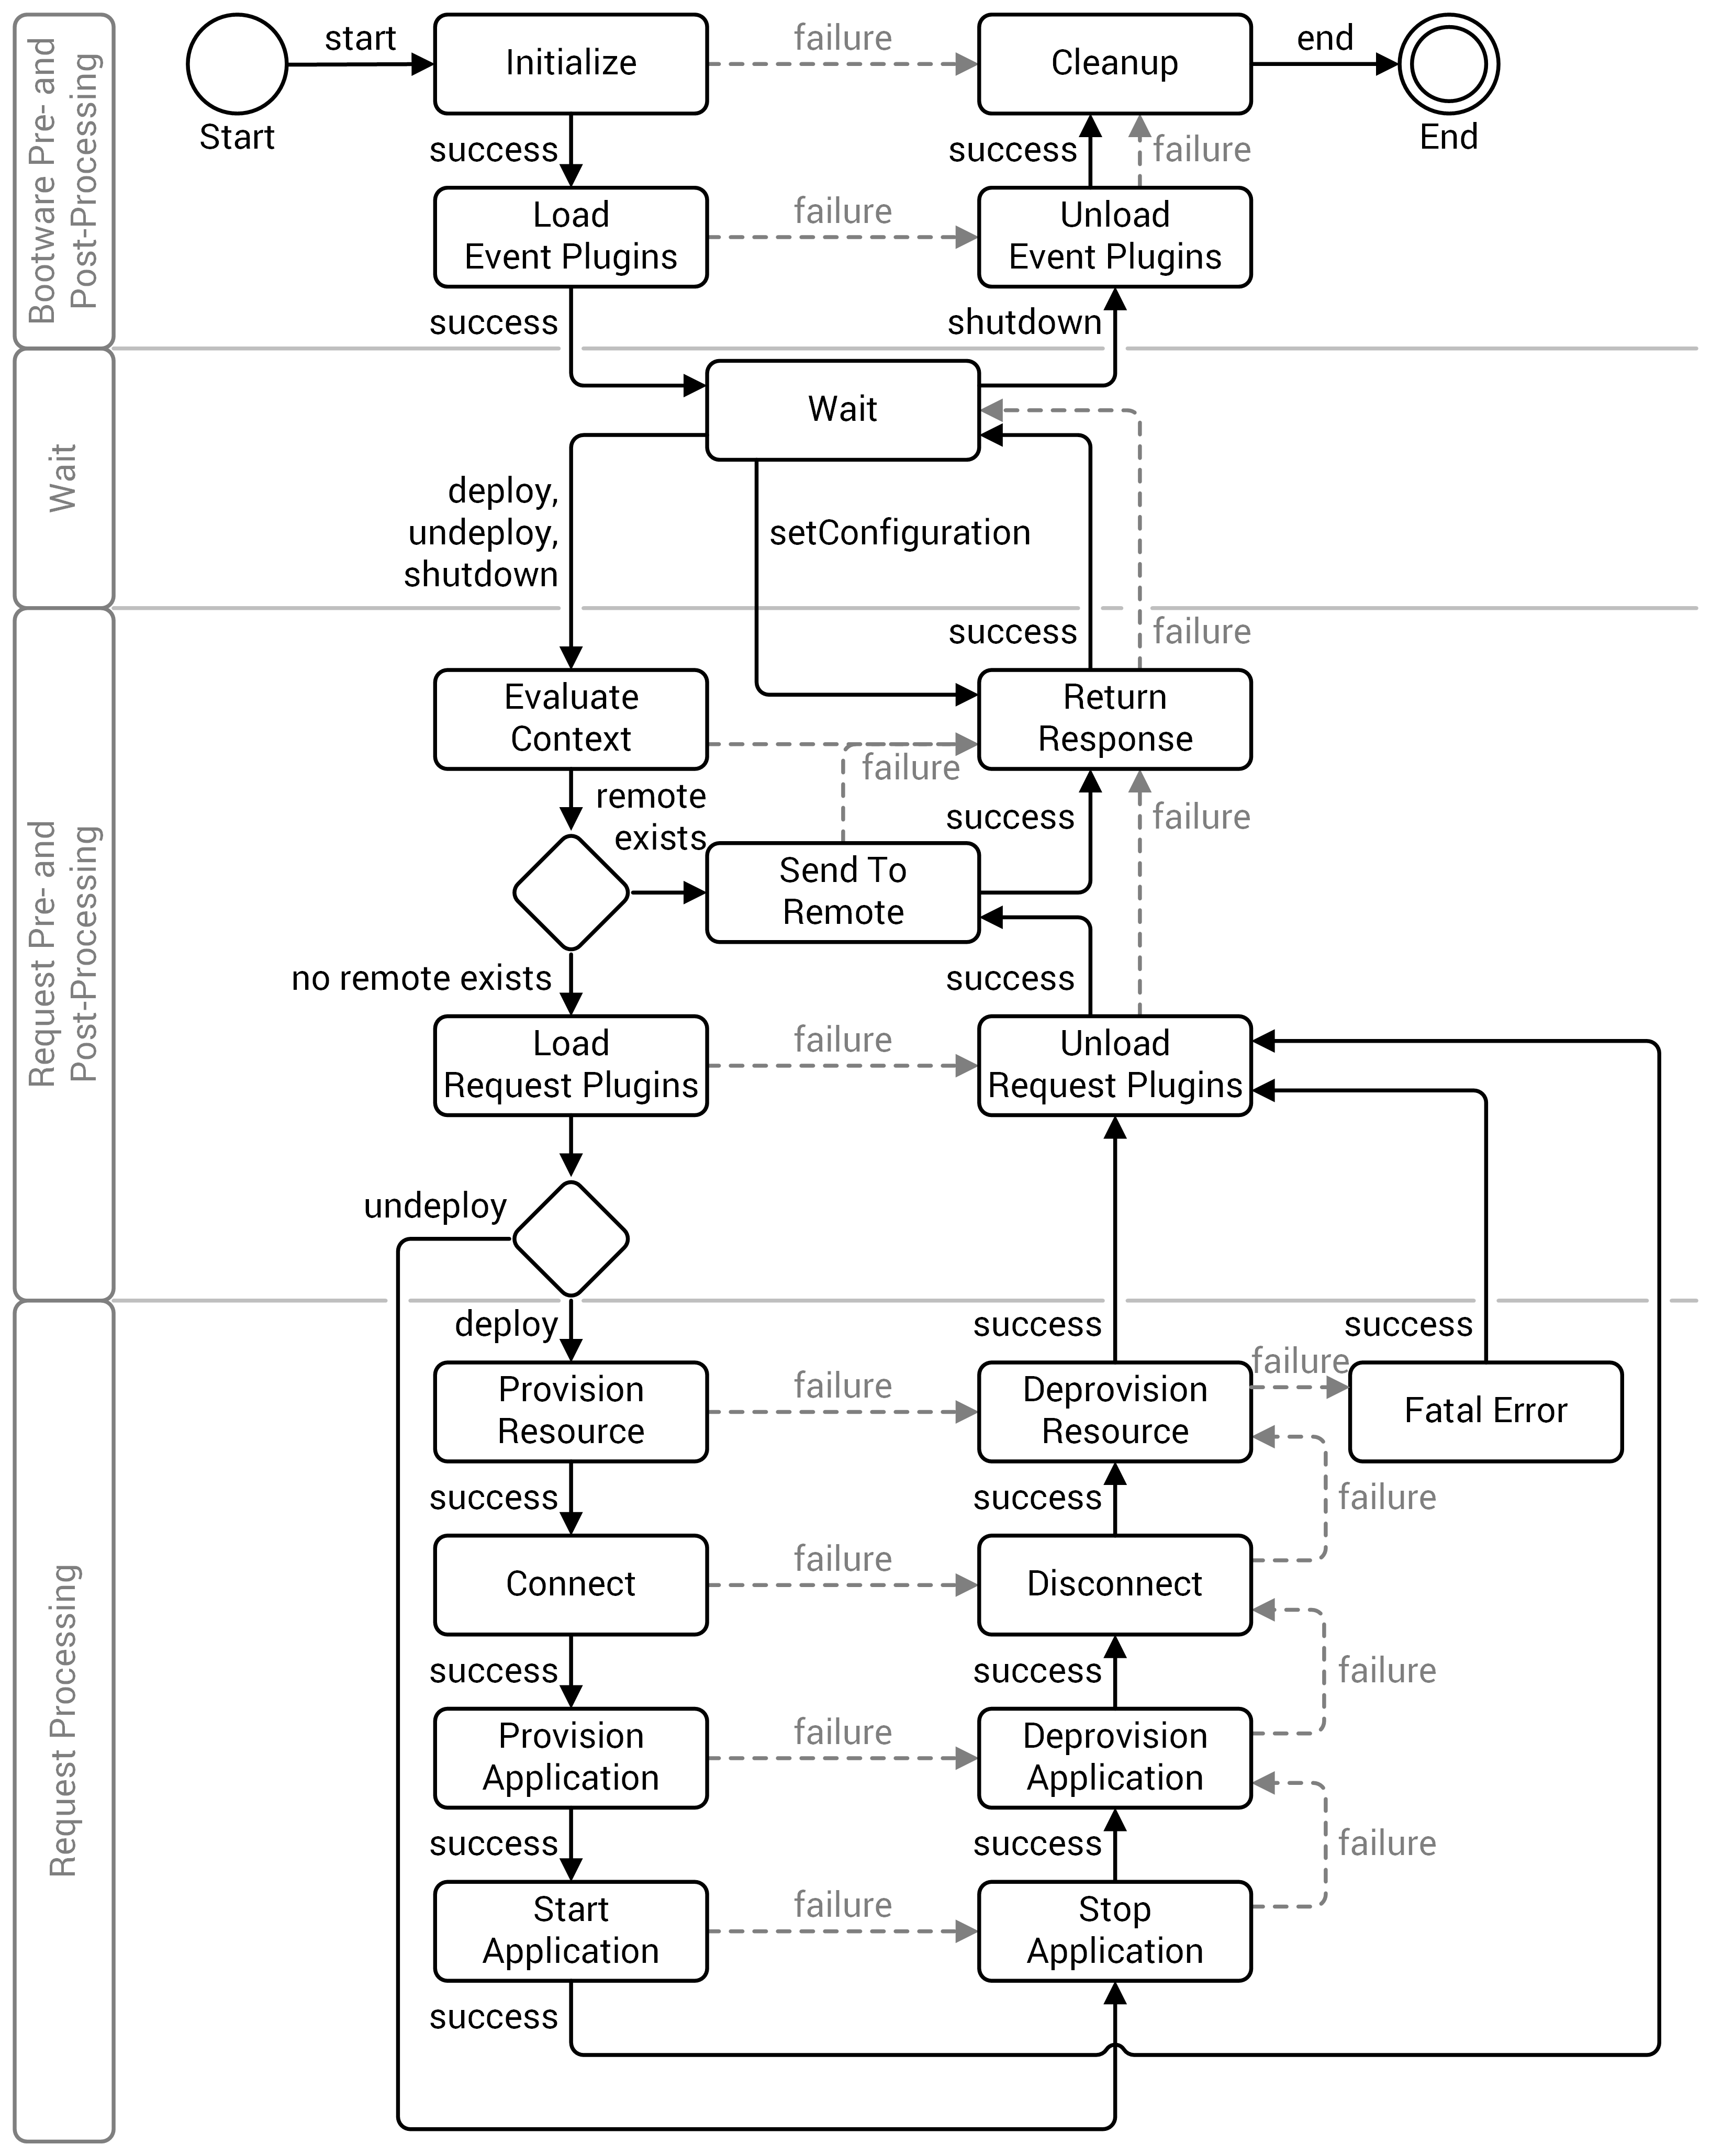
\includegraphics[resolution=600]{design/assets/flow_local}
	\caption{Execution flow in the local bootware.}
	\label{image:flow_local}
\end{figure}

\autoref{image:flow_local} shows a graph that represents the major steps during the bootware execution in the local bootware as flow diagram.
The bootstrapping process is started by executing the local bootware, which is represented by the start state in the top left corner of \autoref{image:flow_local}.
From there, the bootware first does some initializations.
If these fail for some reason, the cleanup code will be executed before the local bootware execution is ended, as can be seen on the top right corner of \autoref{image:flow_local}.
In most cases however, the initialization should succeed.
Then, the local bootware will transition to the next state, where it tries to load the event plugins.

The event plugins are loaded once at the beginning of the local bootware execution, since they will not change at a per request basis (like the other plugins).
If loading one of these plugins fails, the local bootware will try to unload already loaded plugins before continuing to the cleanup state.
If the plugins are loaded successfully, the local bootware transitions into the wait state, shown in the top center of \autoref{image:flow_local}.

Once the local bootware is in the wait state it is ready to receive requests from the outside.
If a shutdown event is received in this state, the local bootware will first call tell the remote bootware to undeploy all active payloads.
Next, the local bootware will undeploy the remote bootware by running through the undeploy process shown on the bottom left with the appropriate plugins.
Then, it will shut itself down by first unloading the event plugins and then running the cleanup code.
This is the only normal way to shutdown the local bootware.
If a request is received in the wait state, the local bootware transitions to the next state, where it reads the request context.

The request context contains all the information necessary to fulfill the request, as described in \autoref{design:context}.
If the context can not be read, the local bootware returns a response containing an error message before returning into the wait state.
If the context is read successfully the local bootware tries to send the request on to the remote bootware, as shown in the middle of \autoref{image:flow_local}.
For this to work, the remote bootware has to exist in the requested remote environment, which won't be the case during the first execution.
Therefore, the local bootware first has to provision the remote bootware in the requested remote environment and so it transitions to the load request plugins state.

In the load request plugins state the plugins specified in the context are loaded.
If this fails, the local bootware tries to unload already loaded plugins before returning an error response and transitioning to the wait state.
If the plugins are loaded successfully, the local bootware now starts either the deploy process or the undeploy process, shown at the bottom of \autoref{image:flow_local}, depending on the type of the request.

If the request was a deploy request, the local bootware will now execute the steps shown in the bottom left of \autoref{image:flow_local} one after another, which include the deploy, connect, and start operations of the infrastructure, connection, and payload plugins.
If one of those operations fails the local bootware transitions over to the corresponding undeploy operation and works its way backwards to undo all operations that where already executed.
This process is the same as the undeploy process, shown on the bottom right of \autoref{image:flow_local}, which is triggered by an undeploy request.

If the stop payload, deprovision payload, or disconnect states fail, the local bootware just continues with the next undeploy state, since these operations are not considered critical.
However, if the deprovision infrastructure state fails, the local bootware transitions to a fatal error state, show at the right of \autoref{image:flow_local}, since this step is considered critical.
This state failing could mean that resources are still active in the cloud and human interaction is necessary to remove them to stop further costs from incurring.
The fatal error state is responsible for taking special actions to remedy this situation.

The successful, as well as the unsuccessful execution of either the deploy or the undeploy process all finish in the unload request plugin state, where the plugins that where needed for this particular request are unloaded.
If everything went as planned, a remote bootware should now be running in the desired cloud environment and the local bootware can now pass on the request to this remote bootware, as shown in the center of \autoref{image:flow_local}.
The local bootware will wait in this state until it receives a response from the remote bootware.

Now, we move our attention to the remote bootware, where the requests continues to be processed.
\autoref{image:flow_remote} shows the execution flow of the remote bootware.
As we can see, it is largely identical to the local bootware, at least at the moment.
The send to remote state is gone, since we don't need this in the remote bootware.
Instead, as the bottom of \autoref{image:flow_remote} shows, the provision and deprovision middleware steps were added.
Other than that, the local and remote processes are the same.

\begin{figure}[!htbp]
	\centering
	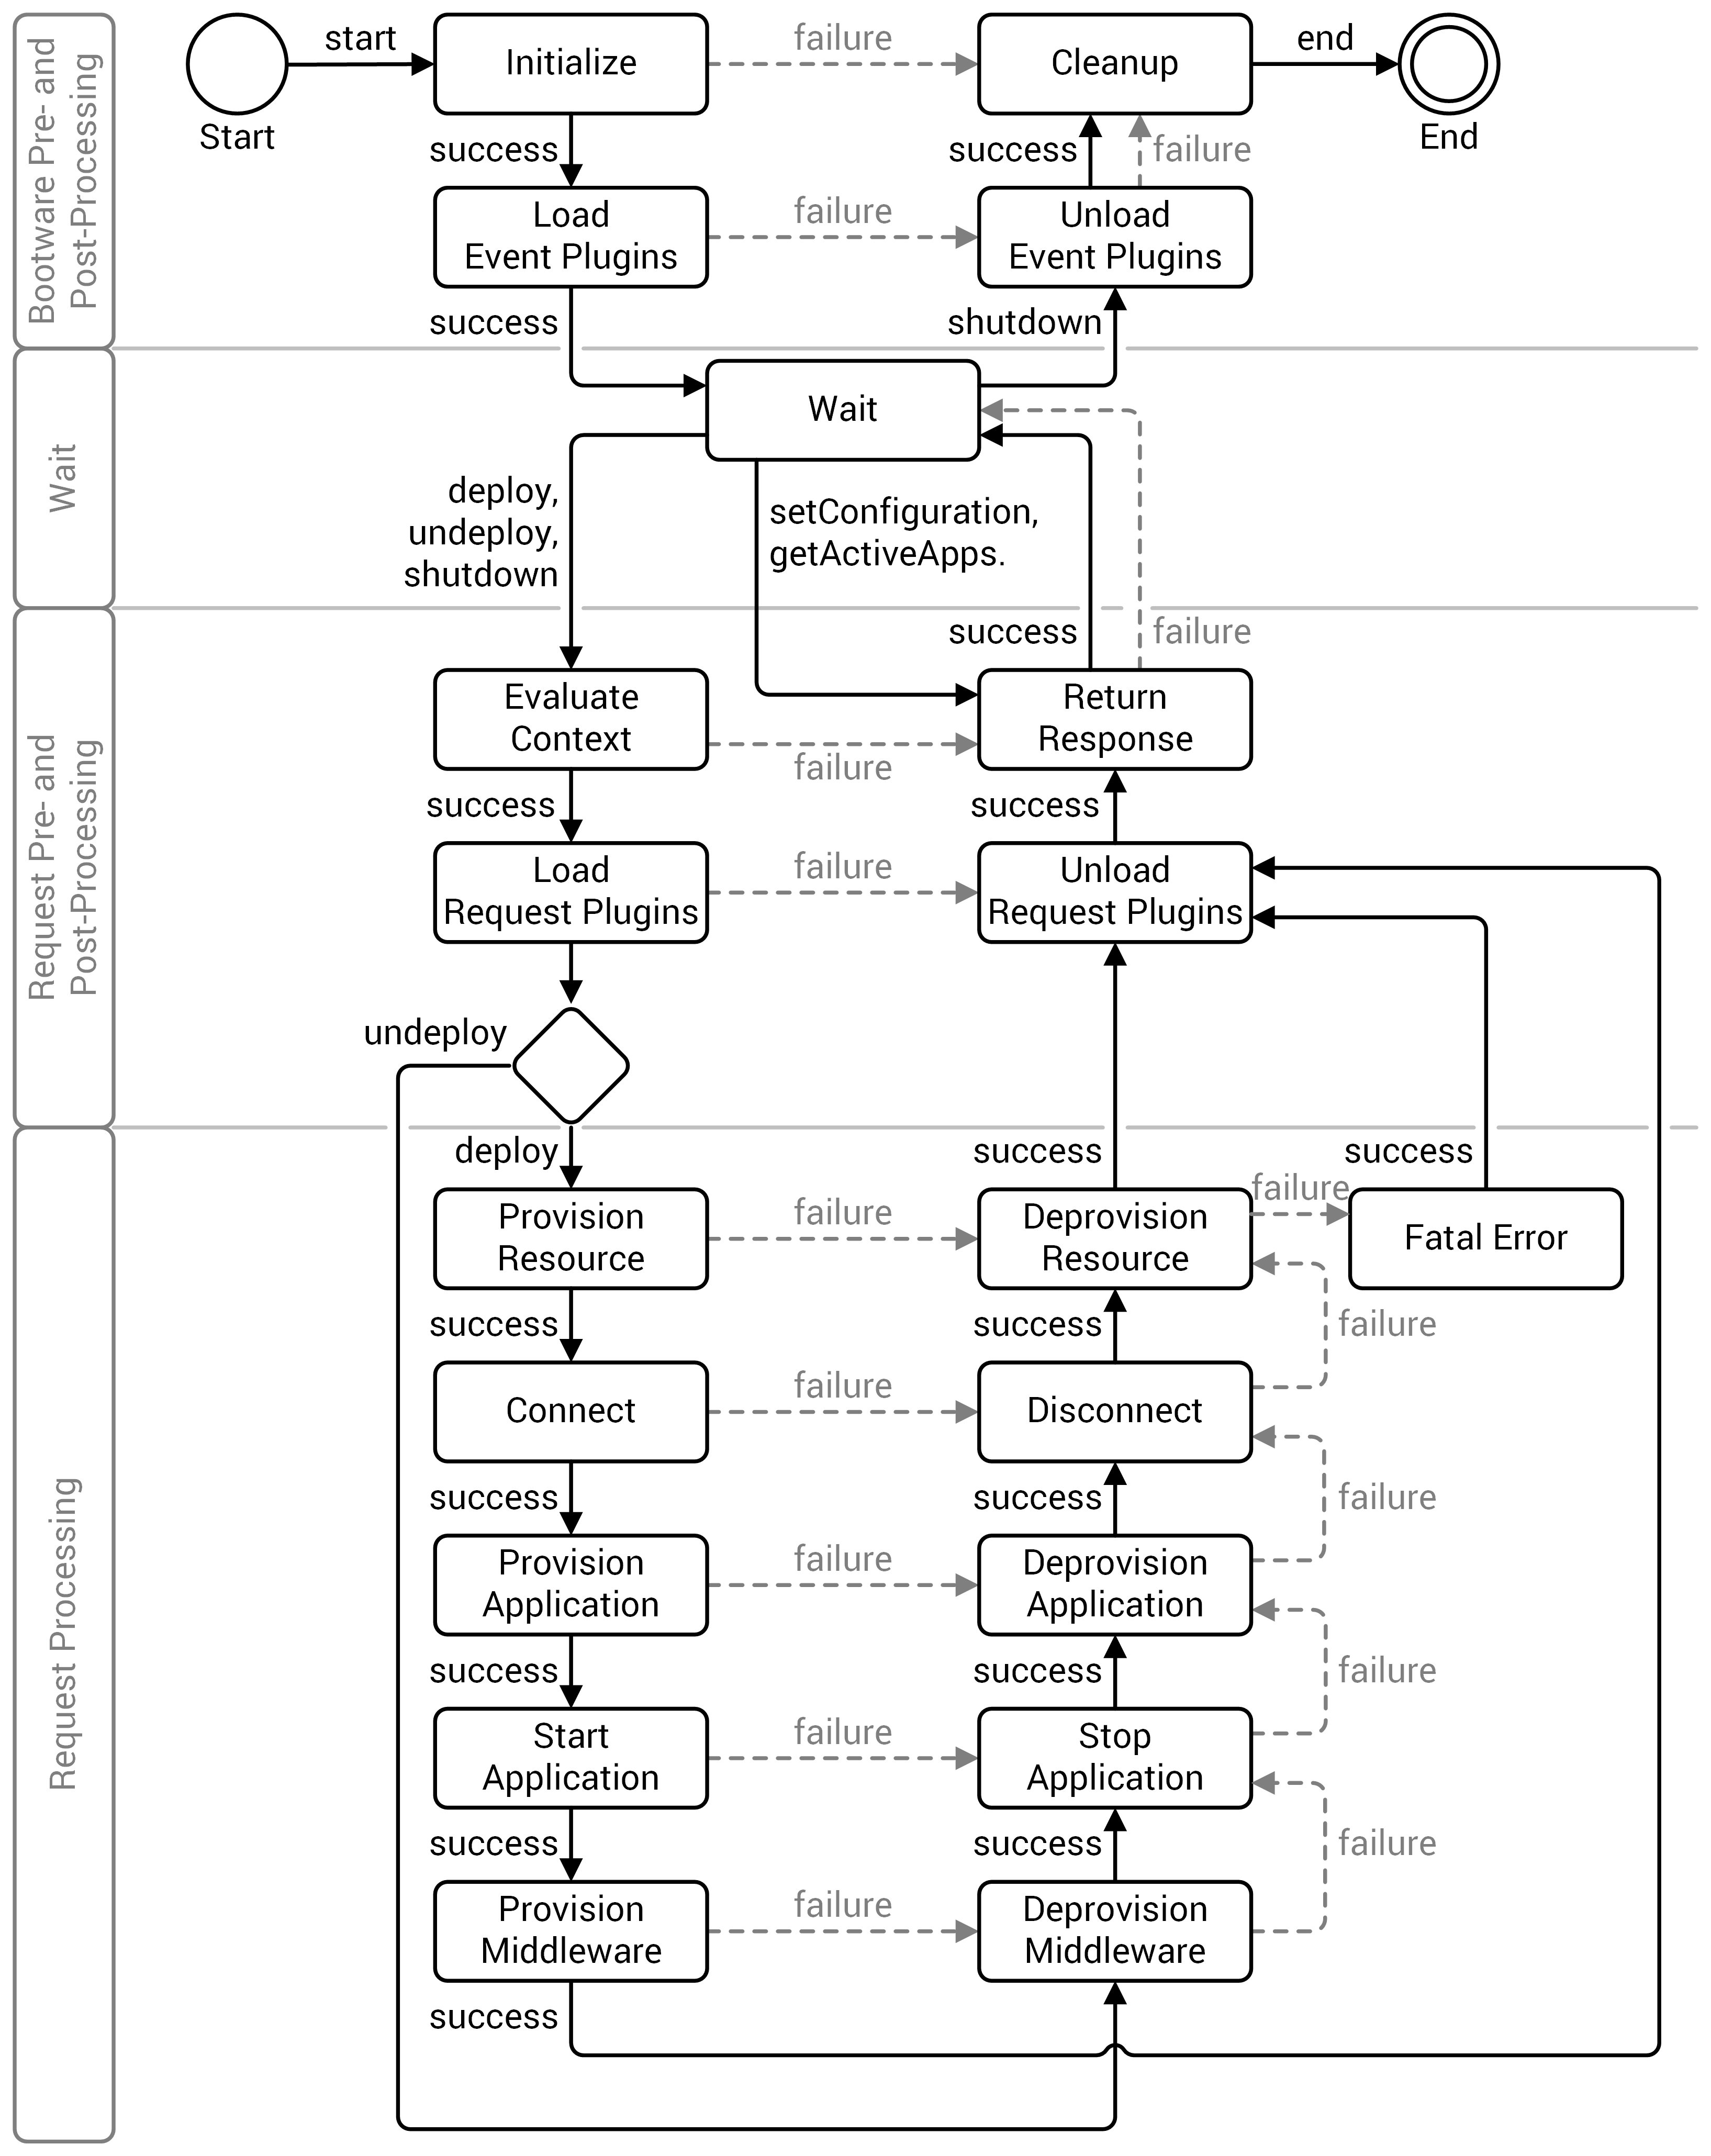
\includegraphics[resolution=600]{design/assets/flow_remote}
	\caption{Execution flow in the remote bootware.}
	\label{image:flow_remote}
\end{figure}

Like the local bootware, the remote bootware went through the initialization steps shown at the top of \autoref{image:flow_remote} when it was started by the local bootware.
It then waited in the wait state for a request.
Now, it receives the request from the local bootware, reads the context, loads the request plugins and executes the deploy operation.
This should result in a provisioning engine being started by the payload plugin.
After that, the remote bootware enters the new provision middleware state at the bottom left of \autoref{image:flow_remote}, which will use the just started provisioning engine to deploy the workflow middleware by executing the provisioning engine plugin.
Once the middleware is running, the remote bootware is finished with this request and returns the endpoint references of the middleware in the response to the local bootware, before returning into the wait state.

This brings us back to \autoref{image:flow_local}, where the local bootware has now received the answer from the remote bootware in the send to remote state.
Now, the local bootware can finish its request by sending back a response to the modeler bootware plugin, before returning to the wait state.
The local bootware is now done until it's time to undeploy the remote bootware.
Meanwhile, the modeler bootware plugin starts the workflow execution on the middleware, during which multiple calls from the provisioning manager to the remote bootware will occur, which will each time trigger the deploy or undeploy process shown at the bottom of \autoref{image:flow_remote}.

As \autoref{image:flow_local}, \autoref{image:flow_remote} and the description above show, this is quite a complicated process with many conditional transition.
Using traditional programming methods like if/else blocks to implement this process would lead to a rather unwieldy and complicated construct with lots of nested if/else block.
Therefore, it could be advantageous to use other methods that are more fitting for this process.
Since we already described the process as a directed graph with states and transition, it would be ideal if we could take this whole graph and use it in the bootware.
Fortunately, this is possible by implementing the process using a finite state machine.

\subsection{Finite State Machine}

In theoretical computer science, a \nom{Finite State Machine}{FSM} is a formal, abstract model of computation that "consisting of a set of states, a start state, an input alphabet, and a transition function that maps input symbols and current states to a next state. Computation begins in the start state with an input string. It changes to new states depending on the transition function"~\autocite{fsm}.
In this context, a state is the "condition of a finite state machine [...] at a certain time. Informally, the content of memory"~\autocite{state}.
The start state is therefore the initial condition of a FSM.
The alphabet is a "set of all possible symbols in an application. For instance, input characters used by a finite state machine, letters making up strings in a language, or symbols in a pattern element. In some cases, an alphabet may be infinite"~\autocite{alphabet}.
The transition function is a "function of the current state and input giving the next state of a finite state machine"~\autocite{transitionfn}.
FSMs can further be distinguished in deterministic and non-deterministic FSMs.
A deterministic FSM has at most one transition for each symbol and state, whereas a non-deterministic FSM can have non, one, or more transitions per symbol and state~\autocite{deterministic}.

Aside from its uses in theoretical computer science, FSMs also have practical applications in digital circuits, software applications, or as lexers in programming language compilers.
We are only interested in the use of FSMs for building software, so we can redefine what a FSM means for our case.
We want to use a FSM as an abstract machine that is defined by a finite list of states and some conditions that trigger transitions between those states.
Unlike a traditional FSM, we will not consume symbols from a set alphabet that will trigger state transitions.
We want the state transitions to be triggered by events that we can emit at any time, so we want an event-driven FSM.
The machine is in only one state at a time, its current state.
At the start of the machine execution, it will be in the start state.
From there, it can transition from one state to another when certain events are triggered, until it finally reaches an end state.
When it enters a state, it executes a function associated with this state.
The result of the execution of this function determines to which state the FSM will transition next.
We will talk more about the actual implementation with FSMs in \autoref{implementation}.

\section{Final Bootware Architecture}
\label{design:finalarch}

\autoref{image:finalarchlocal} and \autoref{image:finalarchremote} show the final architecture of the local and remote bootware component.
Since the only difference between them is the provisioning engine plugin shown in the top right corner of \autoref{image:finalarchremote}, we will describe this figure only.
At the bottom we can see four exemplary event plugins.
These are loaded at the beginning of the bootware execution by the plugin manager, shown on the left of \autoref{image:finalarchremote}.
For demonstrations purposes, \autoref{image:finalarchremote} shows a wider range of possible event plugins.
All these plugins provide some sort of input and/or output mechanism for the bootware component.
A \nom{command-line interface}{CLI} plugin could be used to make the bootware operations accessible via a command-line interface.
A event logger plugin could be used to write all bootware events to a log file.
We can also imagine an event queue plugin that pushes all bootware events into some message queue so that they can be consumed by other components.
Finally, an undeploy trigger plugin could trigger the undeployment of the bootware and all running payloads when it receives a message from the ODE event queue.
Besides the event plugins there is always the web service interface, shown at the bottom right of \autoref{image:finalarchremote}, which provides the standard way to interact with the bootware.

All event plugins and the web service interface work by implementing event handlers for certain events published at the event bus, or by publishing events to the event bus themselves.
As we can see in the center of \autoref{image:finalarchremote}, the event bus and the state machine form the core of the bootware.
The event bus is responsible for distributing events between the various plugins and the state machine.
The state machine implements the entire bootstrapping process, as described earlier in \autoref{design:flow}.
At certain points during the bootstrapping process, operations are delegated to the plugin manager to load plugins, and to the infrastructure, connection, payload, and provisioning engine plugins, shown at the top of \autoref{image:finalarchremote}.

\begin{figure}[!htbp]
	\centering
	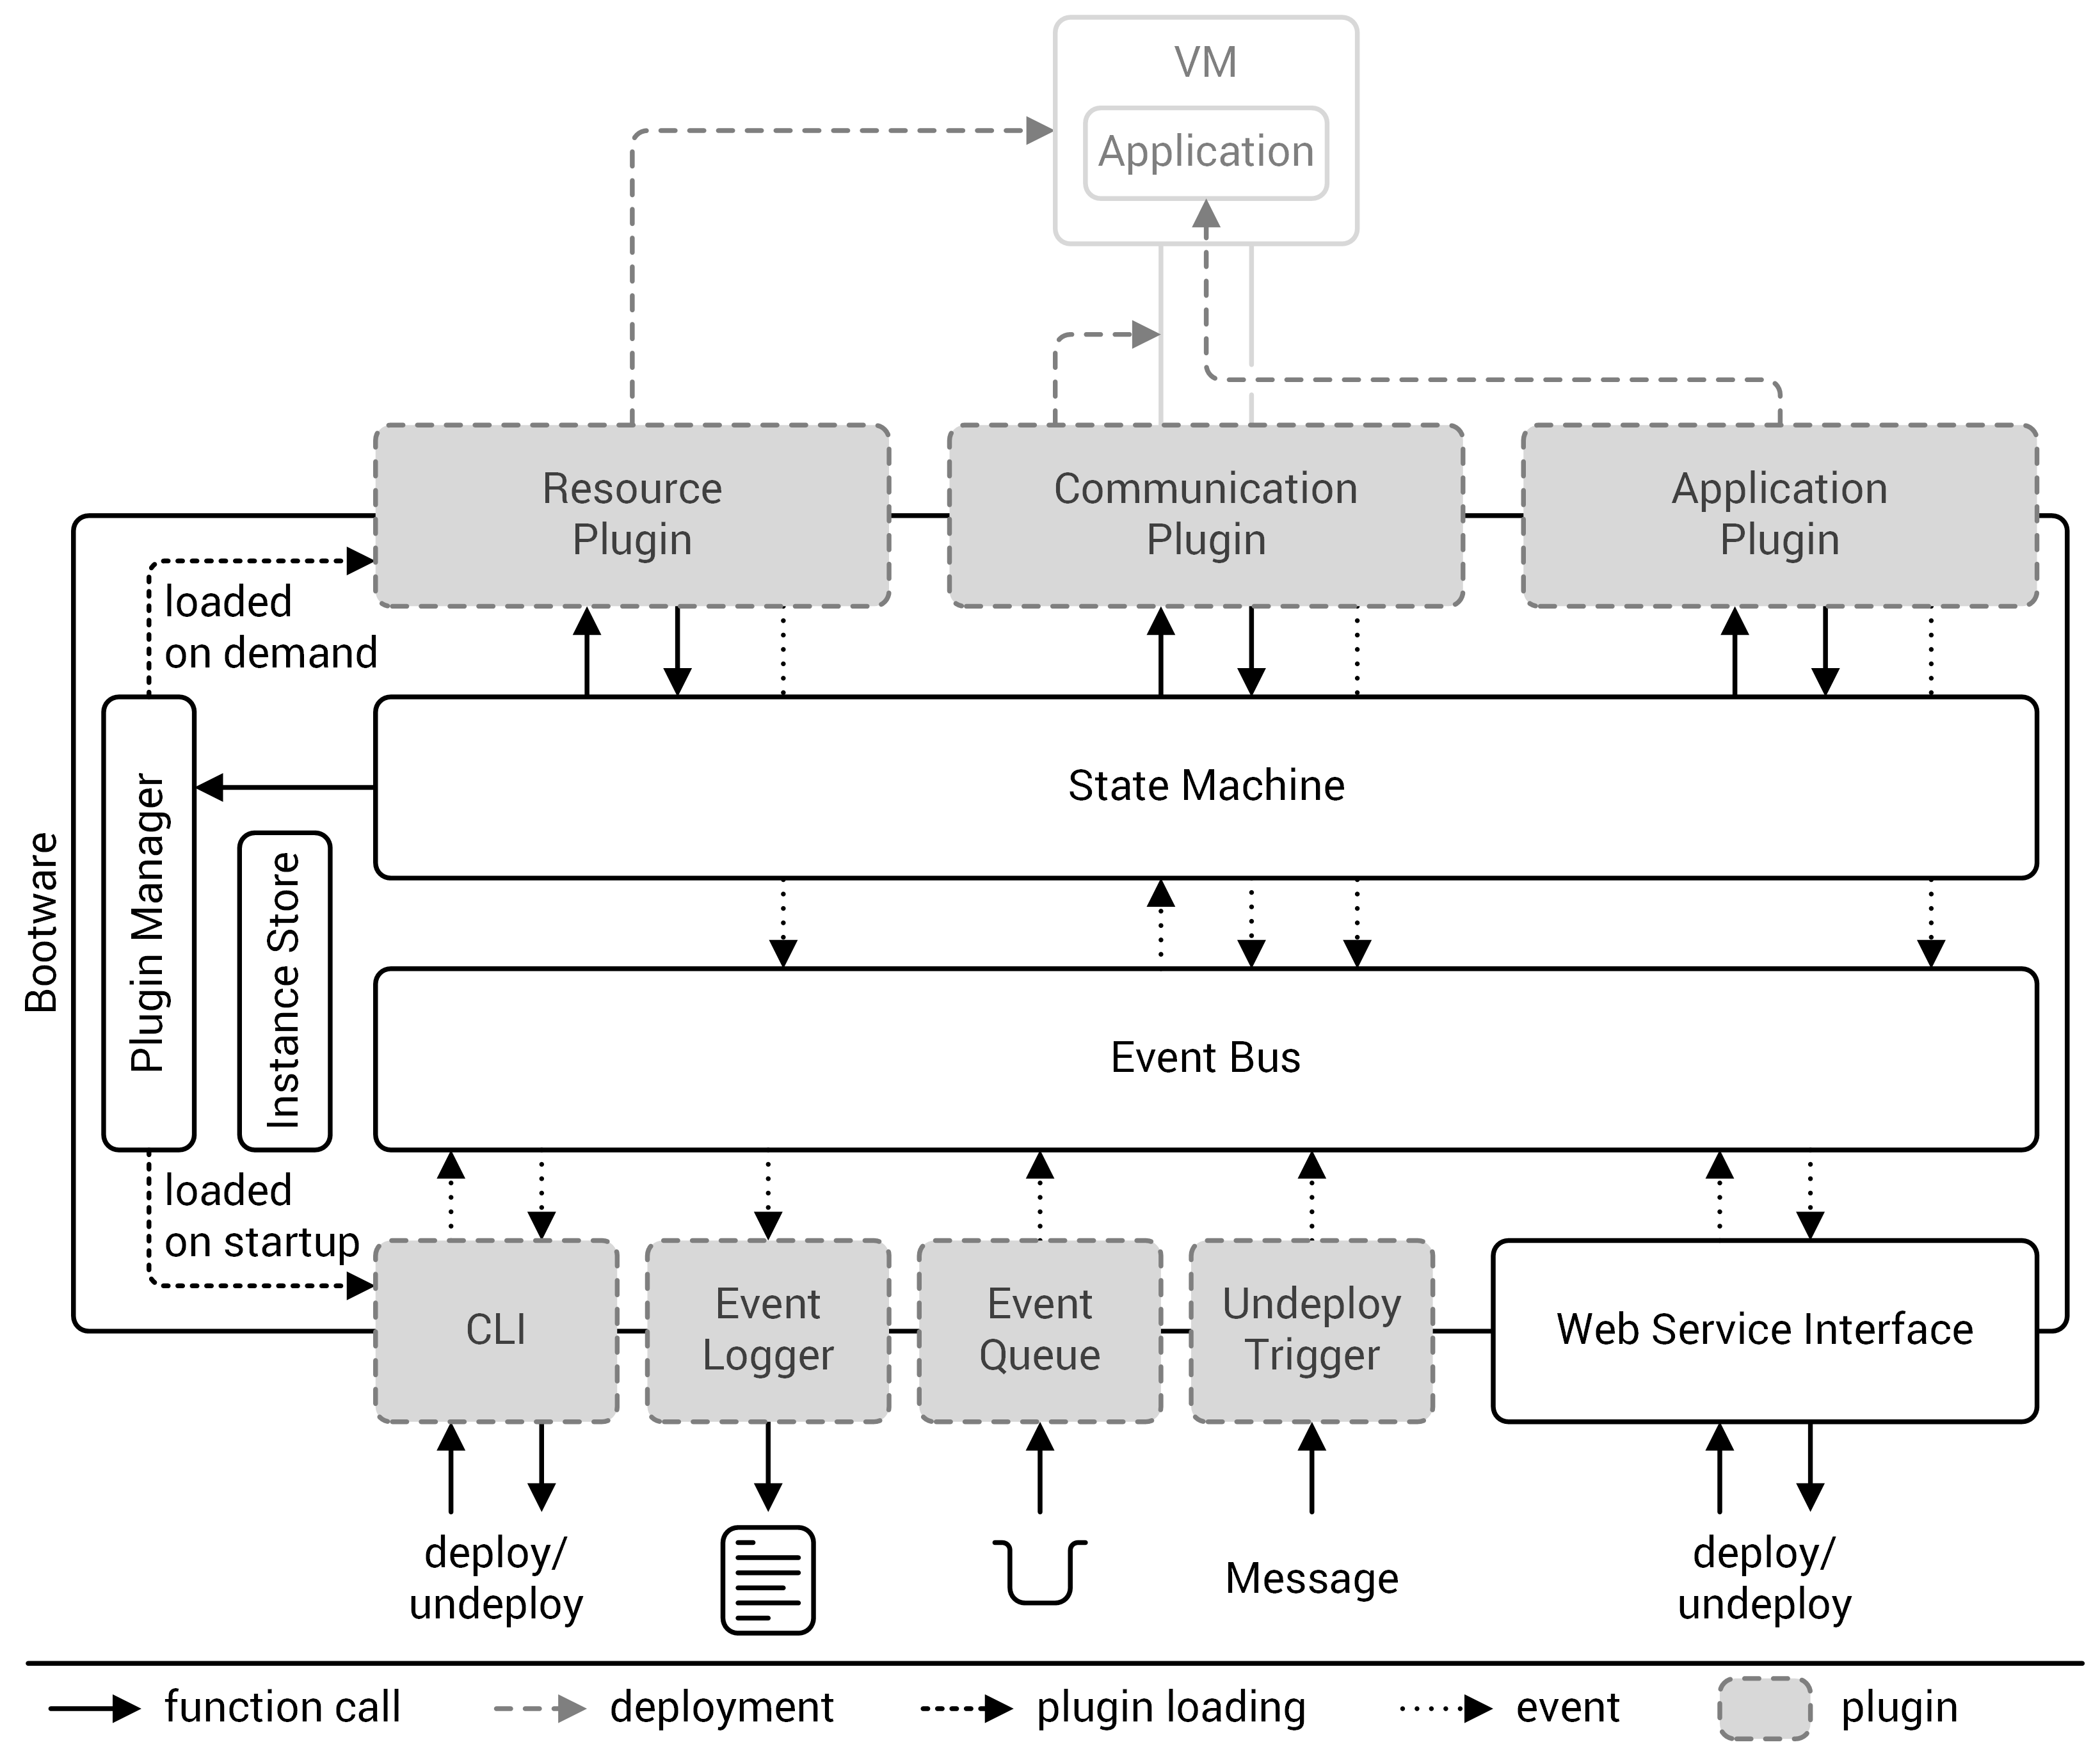
\includegraphics[resolution=600]{design/assets/final_architecture_local}
	\caption{The final architecture of the local bootware component.}
	\label{image:finalarchlocal}
\end{figure}

\begin{figure}[!htbp]
	\centering
	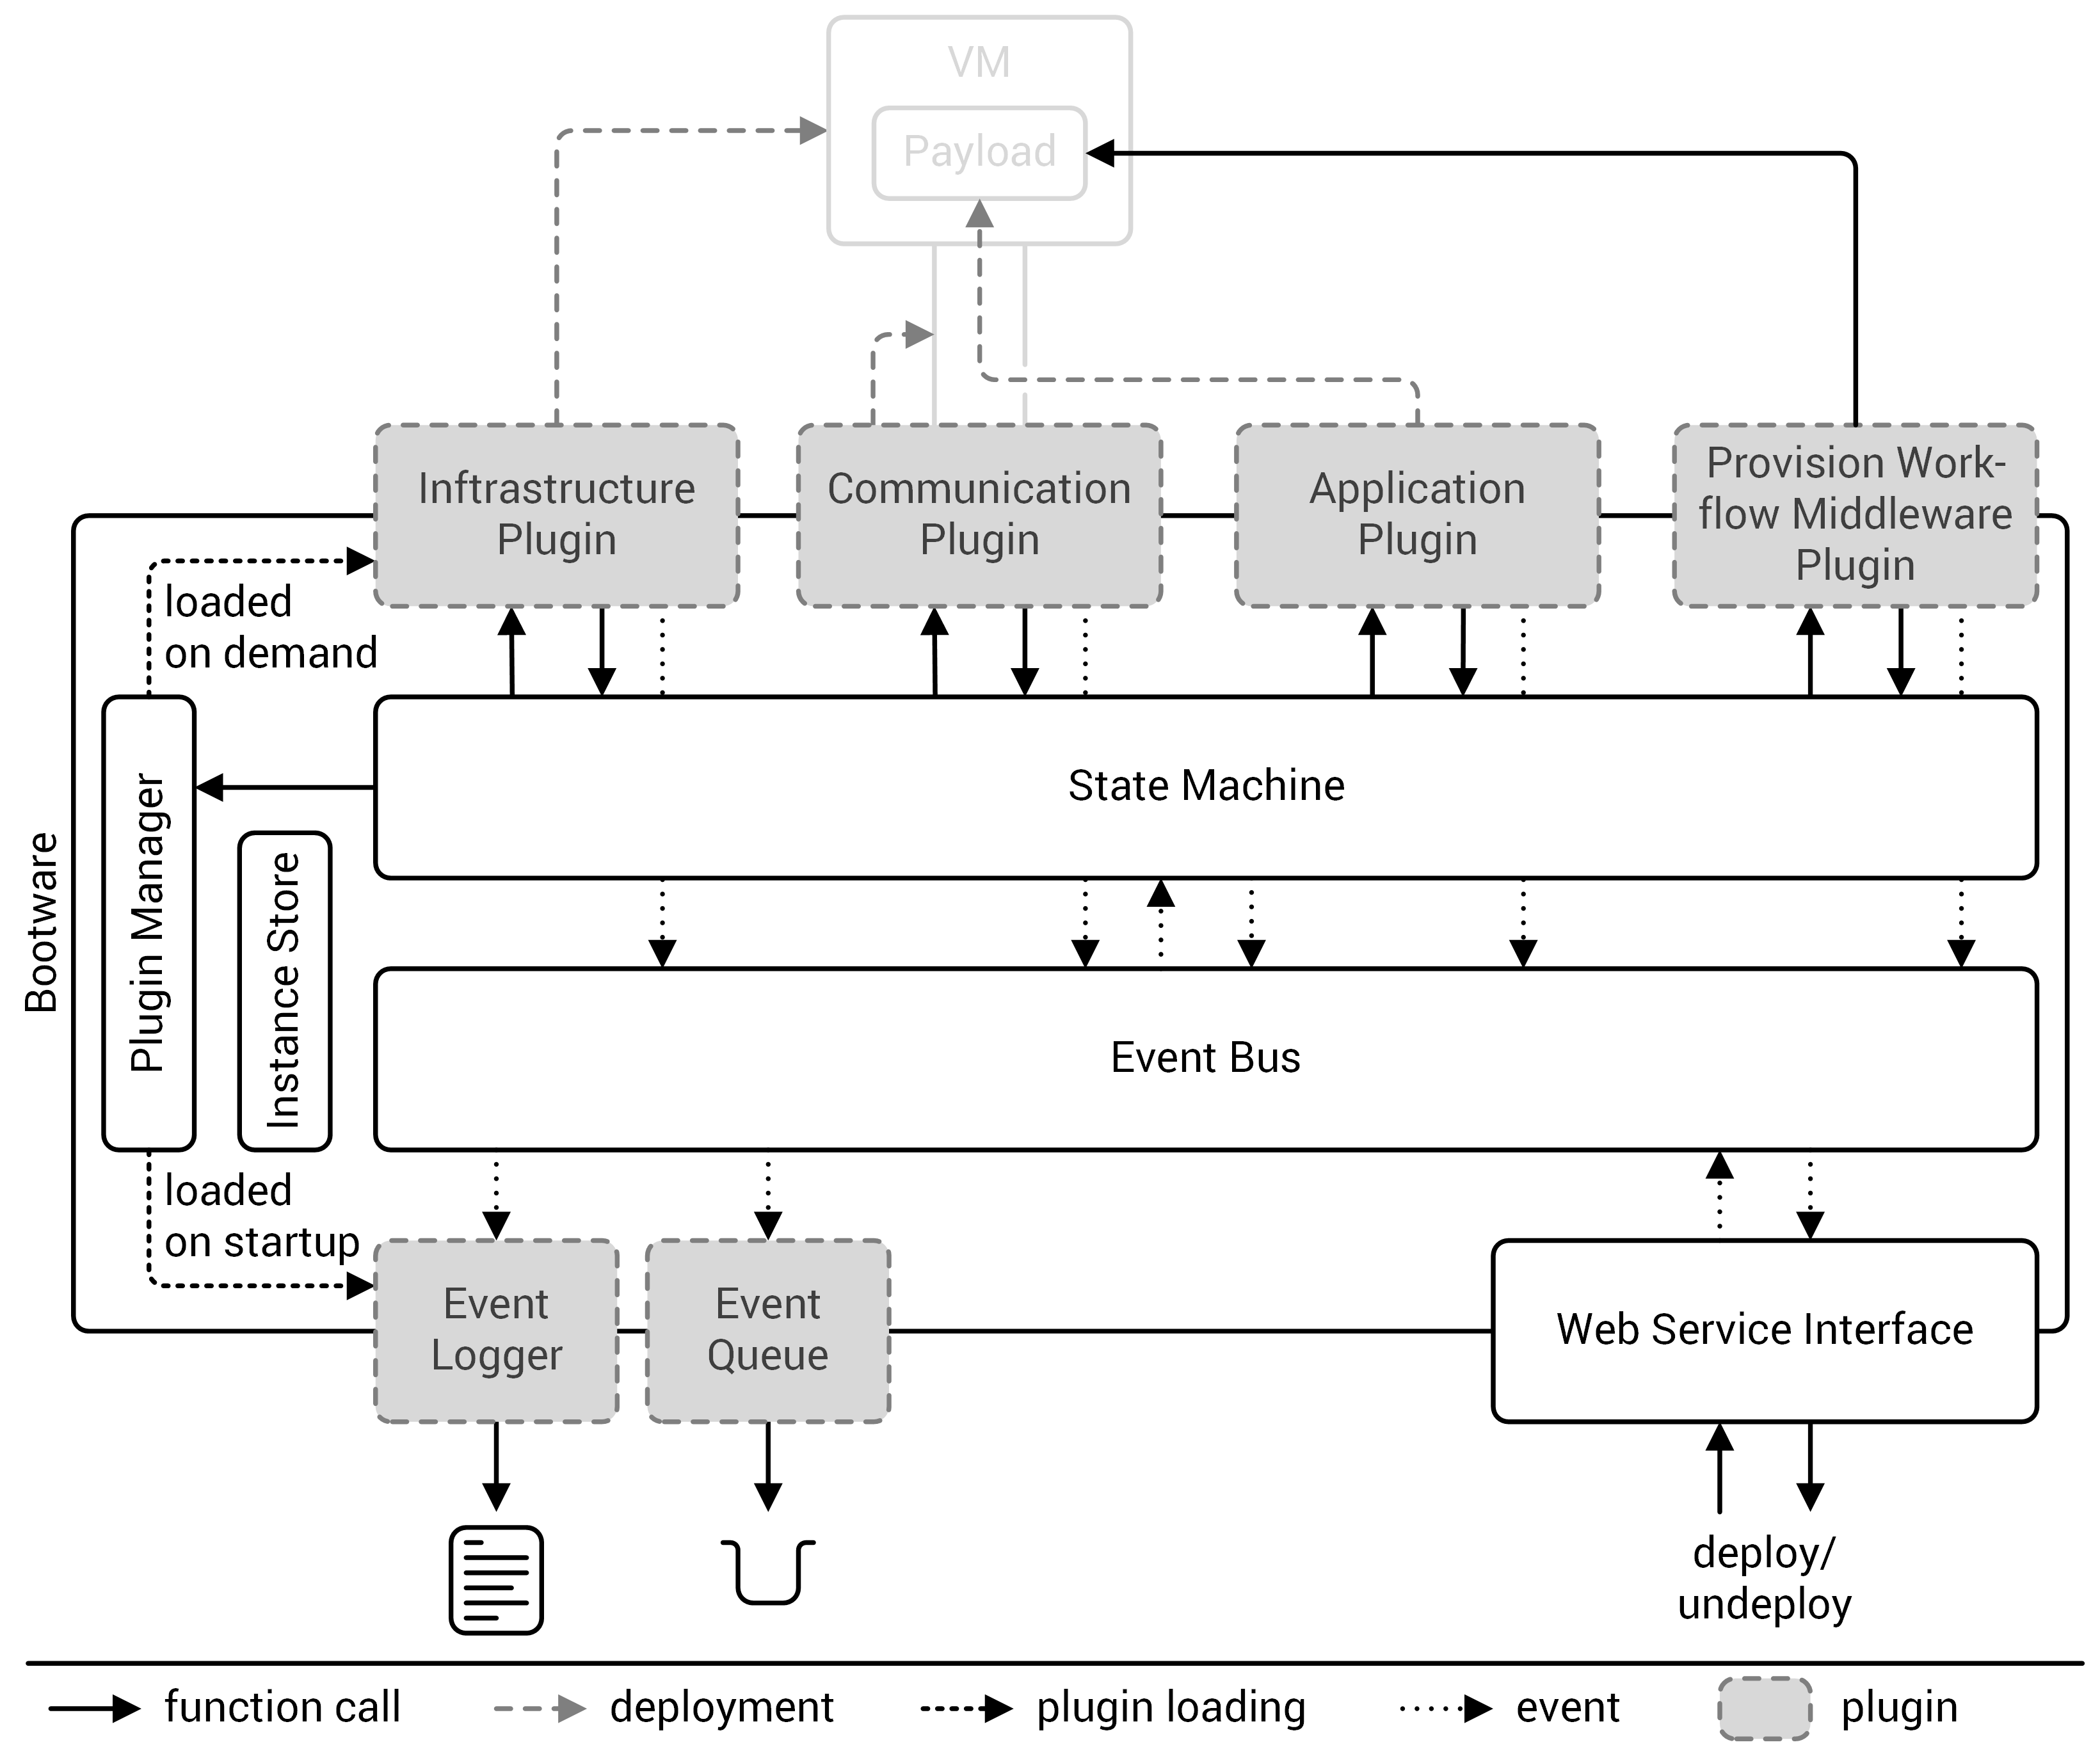
\includegraphics[resolution=600]{design/assets/final_architecture_remote}
	\caption{The final architecture of the remote bootware component.}
	\label{image:finalarchremote}
\end{figure}

The infrastructure, connection, and payload plugins implement the actual bootstrapping operations.
At the top, \autoref{image:finalarchremote} shows an exemplary result of these bootstrapping operations.
In this particular case, the infrastructure plugin started a VM, to which the connection plugin set up a communication channel.
The payload plugin then used this communication channel to provision the payload inside the VM.
The provisioning engine plugin is only available in the remote bootware and allows it to call a provisioning engine with the details necessary to provision the workflow middleware.
This is shown in \autoref{image:finalarchremote} as an additional function call from the provisioning engine plugin to the previously deployed payload.
During the bootstrapping procedure, events are sent from all these plugins back to the event bus to be delivered to the loaded event plugins.

